\thispagestyle{lichsutoanhocnone}
\pagestyle{lichsutoanhoc}
\graphicspath{{../lichsutoanhoc/pic3/}}
\everymath{\color{lichsutoanhoc}}
\blfootnote{$^1$\color{lichsutoanhoc}Viện Toán học, đã nghỉ hưu.}
\blfootnote{$^2$\color{lichsutoanhoc}Hà Nội.}
\begingroup
\AddToShipoutPicture*{\put(0,616){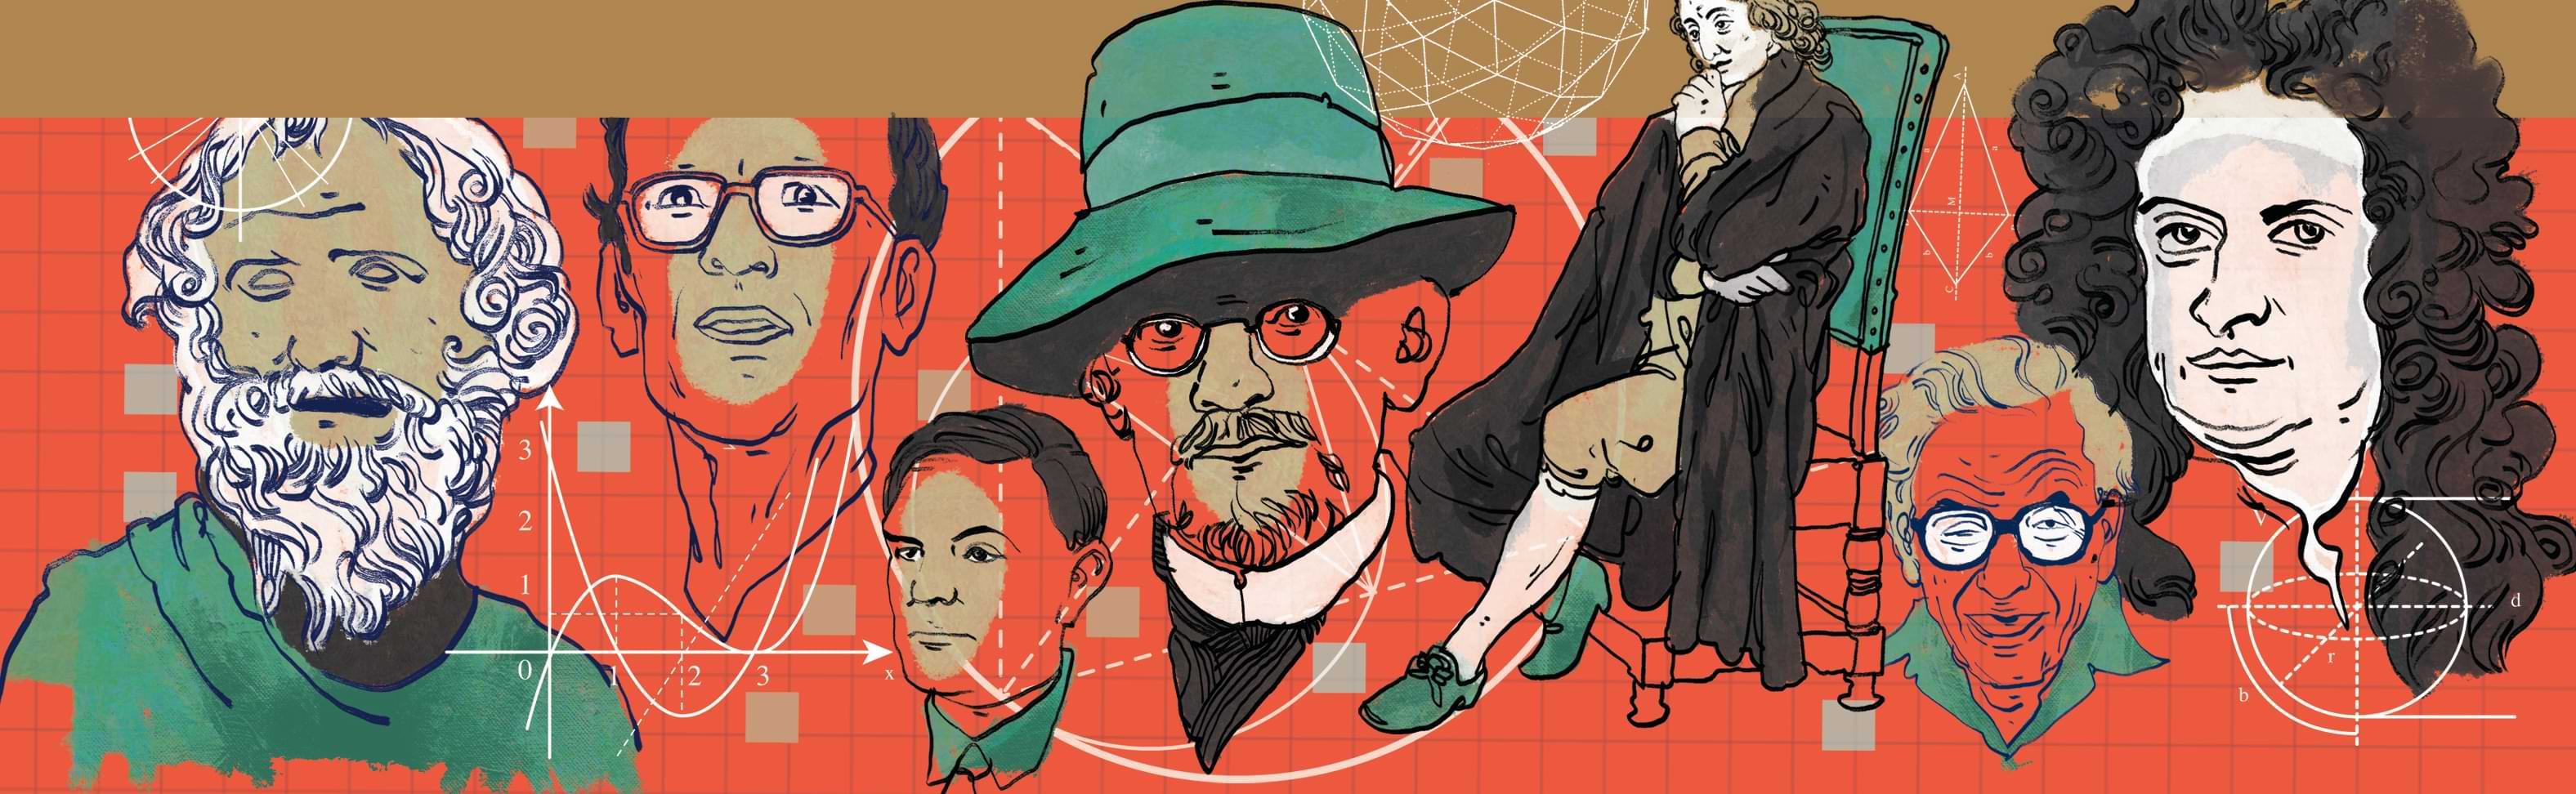
\includegraphics[width=19.3cm]{../bannerlichsu}}}
\AddToShipoutPicture*{\put(56,525){
\includegraphics[scale=1]{../tieude.pdf}}}
\centering
\endgroup

\vspace*{185pt}

\begin{multicols}{2}
	\textbf{\color{lichsutoanhoc}Phụ lục $\pmb1$. Một số công thức tính số} $\pmb{\pi}$ ([$3$])
	\vskip 0.1cm
	$\pmb1$\textbf{\color{lichsutoanhoc}. Archimedes} (khoảng $250$ trước công nguyên)
	\vskip 0.1cm
	Đặt  $P_6 := 4\sqrt{3}, p_6 = 6$ là chu vi lục giác đều ngoại tiếp và nội tiếp đường tròn bán kính $1$ và
	\begin{align*}
		{P_{2n}}: = \frac{{{P_n}{p_n}}}{{{P_n} + {p_n}}}, {p_{2n}}: = \sqrt {{P_{2n}}{p_n}} 
	\end{align*}
	là chu vi đa giác đều ngoại tiếp và nội tiếp đường tròn bán kính $1$ khi gấp đôi số cạnh. Khi ấy (xem [$1$])  $\mathop {\lim }\limits_{n \to \infty } {P_n} = \mathop {\lim }\limits_{n \to \infty } {p_n} = \pi$.
	\vskip 0.1cm
	Nhờ công thức này, Archimedes đã chứng minh được $3\frac{10}{71} < \pi < 3\frac{10}{70}$ và nhà toán học người Áo Christoph Grienberger năm $1630$ đã đạt kỷ lục tính chính xác  số $\pi$  đến $39$ chữ số (xem [$1$]).
	\vskip 0.1cm
	$\pmb2$\textbf{\color{lichsutoanhoc}. Francois Viète} (khoảng $1578$)
	\begin{align*}
		\frac{2}{\pi } =& \sqrt {\frac{1}{2}}  \cdot \sqrt {\frac{1}{2}\left( {1 + \sqrt {\frac{1}{2}} } \right)}  \\
		&\cdot \sqrt {\frac{1}{2}\left( {1 + \sqrt {\frac{1}{2}\left( {1 + \sqrt {\frac{1}{2}} } \right)} } \right)} ...,
	\end{align*}
	Nhờ công thức này, nhà toán học François Viète năm $1578$ đã tính chính xác số $\pi$  đến $9$ chữ số.
	\vskip 0.1cm
	$\pmb3$\textbf{\color{lichsutoanhoc}. John Wallis} (khoảng $1655$)
	\begin{align*}
		\frac{\pi }{2} = \frac{2}{1} \cdot \frac{2}{3} \cdot \frac{4}{3} \cdot \frac{4}{5} \cdot \frac{6}{5} \cdot \frac{6}{7} \cdot \frac{8}{7} \cdot \frac{8}{9}...
	\end{align*}
	$\pmb4$\textbf{\color{lichsutoanhoc}. William Brouncker} (khoảng $1658$)
	\begin{align*}
		\pi  = \frac{4}{{1 + \frac{1}{{2 + \frac{9}{{2 + \frac{{25}}{{2 + ...}}}}}}}}
	\end{align*}
	$\pmb5$\textbf{\color{lichsutoanhoc}. Mādhava, Gregory, Leibnitz} ($1450-1671$)
	\begin{align*}
		\frac{\pi }{2} = 1 - \frac{1}{3} + \frac{1}{5} - \frac{1}{7} + ...
	\end{align*}
	$\pmb6$\textbf{\color{lichsutoanhoc}. Isaac Newton} (khoảng $1666$)
	\begin{align*}
		\pi  =& \frac{{3\sqrt 3 }}{4} \\
		&+\! 24\left(\!\! {\frac{1}{{12}} \!-\! \frac{1}{{5 \!\cdot\! {2^5}}} \!-\! \frac{1}{{28 \!\cdot\! {2^7}}} \!-\! \frac{1}{{72 \!\cdot\! {2^9}}} \!-\! ...}\! \right)
	\end{align*}
	Năm $1665$, Isaac Newton đã tính chính xác số $\pi$ đến $16$ chữ số thập phân.
	\vskip 0.1cm
	$\pmb7$\textbf{\color{lichsutoanhoc}. Công thức kiểu Machin} ($1706-1776$)
	\begin{align*}
		&\frac{\pi }{4} = 4\arctan \left( {\frac{1}{5}} \right) - \arctan \left( {\frac{1}{{239}}} \right);\\
		&\frac{\pi }{4} = \arctan \left( {\frac{1}{2}} \right) + \arctan \left( {\frac{1}{3}} \right);\\
		&\frac{\pi }{4} = 2\arctan \left( {\frac{1}{2}} \right) - \arctan \left( {\frac{1}{7}} \right);\\
		&\frac{\pi }{4} = 2\arctan \left( {\frac{1}{3}} \right) + \arctan \left( {\frac{1}{7}} \right).
	\end{align*}
	Năm $1706$, Machin đã tính chính xác số $\pi$  đến $100$ chữ số thập phân.
	\vskip 0.1cm
	$\pmb8$\textbf{\color{lichsutoanhoc}. Leonard Euler} (khoảng $1748$)
	\begin{align*}
		\frac{{{\pi ^2}}}{6} &= 1 + \frac{1}{{{2^2}}} + \frac{1}{{{3^2}}} + \frac{1}{{{4^2}}} + \frac{1}{{{5^2}}} + ...;\\
		\frac{{{\pi ^4}}}{{90}} &= 1 + \frac{1}{{{2^4}}} + \frac{1}{{{3^4}}} + \frac{1}{{{4^4}}} + \frac{1}{{{5^4}}} + ...;\\
		\frac{{{\pi ^2}}}{6} &= 3\sum\limits_{m = 1}^\infty  {\frac{1}{{{m^2}\left( \begin{array}{l}
						2m\\
						m
					\end{array} \right)}}} .
	\end{align*}
	$\pmb9$\textbf{\color{lichsutoanhoc}. Srinivasa Ramanujan} ($1914$)
	\begin{align*}
		&\frac{1}{\pi } = {\sum\limits_{n = 0}^\infty  {\left( \begin{array}{l}
					2n\\
					n
				\end{array} \right)} ^2}\frac{{42n + 5}}{{{2^{12n + 4}}}};\\
		&\frac{1}{\pi } = \frac{{\sqrt 8 }}{{9801}}\sum\limits_{n = 0}^\infty  {\frac{{\left( {4n} \right)!}}{{{{\left( {n!} \right)}^4}}}} \frac{{\left( {1103 + 26390n} \right)}}{{{{396}^{4n}}}}.
	\end{align*}
	$\pmb10$\textbf{\color{lichsutoanhoc}. Louis Comtet} ($1974$)
	\begin{align*}
		\frac{{{\pi ^4}}}{{90}} = \frac{{36}}{{17}}\sum\limits_{m = 1}^\infty  {\frac{1}{{{m^4}\left( \begin{array}{l}
						2m\\
						m
					\end{array} \right)}}.} 
	\end{align*}
	$\pmb11$\textbf{\color{lichsutoanhoc}. Eugene Salamin, Richard Brent} ($1976$)
	\vskip 0.1cm
	Đặt $a_0 := 1, b_0 = \frac{1}{\sqrt{2}}, s_0 = \frac{1}{2}$.
	\vskip 0.1cm     
	Với $k = 1,2,3, \ldots$ tính 
	\begin{align*}
		&{a_k} = \frac{{{a_{k - 1}} + {b_{k - 1}}}}{2}, {b_k} = \sqrt {{a_{k - 1}}{b_{k - 1}}} ,\\
		& {c_k} = a_k^2 - b_k^2, {s_k} = {s_{k - 1}} - {2^k}{c_k}, \\
		&{p_k} = \frac{{2a_k^2}}{{{s_k}}}.
	\end{align*}
	Khi ấy $\mathop {\lim }\limits_{k \to \infty } {p_k} = \pi$   và tốc độ hội tụ là cấp hai. 
	\vskip 0.1cm
	$\pmb{12.}$ \textbf{\color{lichsutoanhoc}Ronathan Borwein, Peter Borwein} ($1985$)
	\vskip 0.1cm
	Đặt ${a_0} = 6 - 4\sqrt 2 ,\;{y_0} = \sqrt 2  - 1.$  
	\vskip 0.1cm
	Với $k = 1,2,3,\ldots$ tính 
	\begin{align*}
		{y_{k + 1}} =& \frac{{1 - \sqrt[4]{{1 - y_k^4}}}}{{1 + \sqrt[4]{{1 - y_k^4}}}},\\
		{a_{k + 1}} =& {a_k}{\left( {1 + {y_{k + 1}}} \right)^4} \\
		&- {2^{2k + 3}}{y_{k + 1}}\left( {1 + {y_{k + 1}} + y_{k + 1}^2} \right).
	\end{align*}
	Khi ấy $\mathop {\lim }\limits_{k \to \infty } {a_k} = \frac{1}{\pi }$  và tốc độ hội tụ là cấp hai.
	\vskip 0.1cm
	$\pmb{13.}$ \textbf{\color{lichsutoanhoc}Ronathan Borwein, Peter Borwein} ($1985$)
	\vskip 0.1cm
	Hệ thức sau đây không đúng nhưng chính xác đến $42$ tỷ chữ số thập phân
	\begin{align*}
		\pi  = {\left( {\frac{1}{{{{10}^5}}}\sum\limits_{n =  - \infty }^\infty  {{e^{ - \frac{{{n^2}}}{{{{10}^{10}}}}}}} } \right)^2}.
	\end{align*}
	$\pmb{14.}$ \textbf{\color{lichsutoanhoc}David Chudnovsky, Gregory Chudnovsky} ($1989$)
	\begin{align*}
		\frac{1}{\pi } =& 12\sum\limits_{n = 0}^\infty  {{{\left( { - 1} \right)}^n}\frac{{\left( {6n} \right)!}}{{{{\left( {n!} \right)}^3}\left( {3n} \right)!}}} \\
		&\times\frac{{13591409 + n545140134}}{{{{\left( {{{640320}^3}} \right)}^{n + \frac{1}{2}}}}}.
	\end{align*}
	$\pmb{15.}$ \textbf{\color{lichsutoanhoc}Ronathan Borwein, Peter Borwein} ($1989$)
	\begin{align*}
		\frac{1}{\pi } = 12\sum\limits_{n = 0}^\infty  {\frac{{{{\left( { - 1} \right)}^n}\left( {6n} \right)!}}{{{{\left( {n!} \right)}^3}\left( {3n} \right)!}}} \frac{{\left( {A + nB} \right)}}{{{C^{n + \frac{1}{2}}}}}.
	\end{align*}
	Trong đó 
	\begin{align*}
			A\!:\! &\!=\! 212175710912\sqrt {61}  \!+\! 1657145277365;\\
			B\!:\! &\!=\! 13773980892672\sqrt {61}  \!+\! 107578229802750;\\
			C\!:\! &\!=\! {\left[ {5280\left( {236674 + 30303\sqrt {61} } \right)} \right]^3}.
	\end{align*}
	$\pmb{16.}$ \textbf{\color{lichsutoanhoc}Ronathan Borwein, Peter Borwein} ($1991$)
	Đặt $a_0 = \frac{1}{3}, s_0 = \frac{\sqrt{3} -1}{2}$.
	\vskip 0.1cm  
	Với $k = 1,2,3, \ldots$ tính 
	\begin{align*}
		&{r_{k + 1}} = \frac{3}{{1 + 2\sqrt[3]{{1 - s_k^3}}}}, {s_{k + 1}} = \frac{{{r_{k + 1}} - 1}}{2},\\
		&{a_{k + 1}} = r_{k + 1}^2{a_k} - {3^k}\left( {r_{k + 1}^2 - 1} \right)
	\end{align*}
	Khi ấy $\mathop {\lim }\limits_{k \to \infty } \frac{1}{{{a_k}}} = \pi $   và tốc độ hội tụ là cấp ba.
	\vskip 0.1cm
	$\pmb{17.}$ \textbf{\color{lichsutoanhoc}David Bailey, Peter Borwein và Simon Plouffe} ($1996$)
	\begin{align*}
		\pi  \!=\!\!\! \sum\limits_{i = 0}^\infty  {\frac{1}{{{{16}^i}}}\!\!\left(\!\! {\frac{4}{{8i \!+\! 1}} \!-\! \frac{2}{{8i \!+\! 4}} \!-\! \frac{1}{{8i \!+\! 5}} \!-\! \frac{1}{{8i \!+\! 6}}} \!\right).}
	\end{align*}
	Các công thức trên là cơ sở để tính gần đúng số $\pi$  trên máy tính điện tử.
	\vskip 0.1cm
	\textbf{\color{lichsutoanhoc}Tính gần đúng số $\pmb{\pi}$  trên máy tính điện tử}
	\vskip 0.1cm
	Lần đầu tiên số $\pi$  được tính gần đúng đến $2037$ chữ số mất $70$ giờ, theo công thức Marchin ($6$), trên máy tính điện tử ENIAC (Electronic Numerical Integrator and Computer) tại phòng nghiên cứu Ballistic vào tháng $9$ năm $1949$.
	Tháng $11$ năm $1954$ và tháng $1$ năm $1955$, Naval Ordnance Reseach Calculator tại Dahlgren, bang Virgina (Mỹ) đã tính gần đúng số  $\pi$ đến $3089$ chữ số trong $13$ phút.
	\vskip 0.1cm
	Kỷ lục này đã bị phá vỡ vào tháng $3$ năm $1957$ khi máy tính Pegasus tại Ferranti Computer Centre (London) tính được $10021$ chữ số trong $33$ giờ. Tuy nhiên, chỉ có $7480$ chữ số chính xác.
	\vskip 0.1cm
	Tháng $6$ năm $1958$, máy tính IBM $704$ tại Paris Data Processing Center đã tính được $10000$ chữ số trong vòng $1$ giờ $40$ phút nhờ chương trình được lập trên sự kết hợp công thức Machin ($6$) và chuỗi Gregory -- Leibnitz ($4$).
	\vskip 0.1cm
	Một năm sau, vào tháng $7$ năm $1959$, máy tính IBM $704$ tại Commissariat à l'Enrgie Atomique (Paris) đã tính được $16167$ chữ số trong vòng $4$ giờ $20$ phút, cũng theo chương trình trên.
	\vskip 0.1cm
	Công thức Machin cũng là cơ sở để máy tính IBM $7090$ tại the London Data Centre chạy chương trình vào tháng $7$ năm $1961$ với kết quả $20000$ chữ số mất $39$ phút.
	\vskip 0.1cm
	Vào thời điểm này, bộ nhớ máy tính gần như đã đạt đến giới hạn. Để đạt được độ chính xác cao hơn, có thể khéo léo sửa đổi chương trình để sử dụng thời gian chạy máy lâu hơn, nhưng như vậy lại phải chịu những chi phí không hợp lý.
	\vskip 0.1cm
	Vào tháng $7$ năm $1961$, Shanks và Wrench đã tăng tốc độ tính toán lên gấp $20$ lần. Điều này một phần do IBM Data Processing Center (New York) đã sử dụng IBM $7090$ có tốc độ nhanh, một phần họ đã sử dụng công thức được Stömer tìm ra năm $1896$, thay cho công thức Machin:
	\begin{align*}
		\pi  =& 24\arctan \frac{1}{8} + 8\arctan \frac{1}{{57}} \\
		&+ 4\arctan \frac{1}{{239}} \tag{$11$}
	\end{align*}
	Sau $8$ giờ $43$ phút, máy đã tính được $100265$ chữ số và $100000$ chữ số đầu đã được in ra trên $20$ tờ giấy A$4$, mỗi tờ có $5000$ chữ số.
	\vskip 0.1cm
	Sau đó, vào tháng $2$ năm $1966$ trên IBM $7030$ và một năm sau, vào tháng $2$ năm $1967$, máy CDC $6600$ tại Commissariat à l'Enrgie Atomique (Paris) đã tính được $500000$ chữ số dựa trên công thức Stömer ($11$), mất $29$ giờ $45$ phút chạy chương trình và $16$ giờ $35$ phút kiểm tra. 
	\vskip 0.1cm
	Nhà toán học Nhật Bản Yasumasa Kanada lập nhiều kỷ lục về tính gần đúng số   trong khoảng $1995-2002$, ông đã tính được gần đúng số  $\pi$ đến trên $1$ nghìn tỷ chữ số thập phân.
	\vskip 0.1cm
	Năm $2019$, nhà khoa học máy tính người Nhật Emma Haruka Iwao đã lập kỷ lục thế giới khi đã tính được hơn $31{,}4$ nghìn tỷ chữ số của $\pi$.
	\vskip 0.1cm 
	Sử dụng máy tính hiệu năng cao, vào ngày $19$ tháng $8$ năm $2021$, một nhóm các nhà nghiên cứu Thụy Sĩ đã tính được giá trị gần đúng mới của $\pi$  gồm $62.831.853.071.796$ chữ số.
	\vskip 0.1cm
	Ngày $21$ tháng $3$ năm $2022$, Google Cloud thông báo rằng họ vừa lập kỷ lục thế giới mới tính giá trị gần đúng của $\pi$  đến $100$ nghìn tỷ chữ số, đánh bại kỷ lục trước đó là $62{,}8$ nghìn tỷ.
	\vskip 0.1cm
	\textbf{\color{lichsutoanhoc}Phụ lục $\pmb2$ Các mốc thời gian tính số $\pmb{\pi}$ }([$3$])
	\begin{figure}[H]
		\vspace*{-5pt}
		\centering
		\captionsetup{labelformat= empty, justification=centering}
		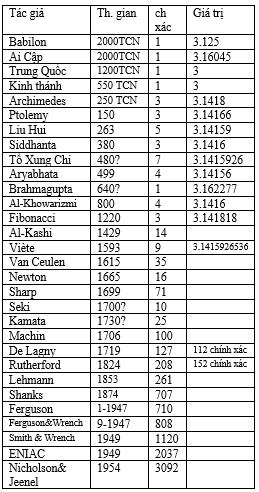
\includegraphics[width= 1\linewidth]{4}
%		\caption{\small\textit{\color{}}}
		\vspace*{-10pt}
	\end{figure}
%%	\vskip 0.1cm
%%	\begin{tabular}{|l|c|c|l}
%%		\hline
%%		Tác giả &	Th. gian&	chuẩn xác&	Giá trị\\
%%		\hline
%%		Babilon&	$2000$TCN&	$1$&	$3.125$\\
%%		\hline
%%		Ai Cập& 	$2000$TCN&	$1$&	$3.16045$\\
%%		\hline
%%		Trung Quốc&	$1200$TCN&	$1$&	$3$\\
%%		\hline
%%		Kinh thánh&	$550$ TCN&	$1$&	$3$\\
%%		\hline
%%		Archimedes&	$250$ TCN&	$3$&	$3.1418$\\
%%		\hline
%%		Ptolemy	&$150$&	$3$&	$3.14166$\\
%%		\hline
%%		Liu Hui	&$263$&	$5$&	$3.14159$\\
%%		\hline
%%		Siddhanta&	$380$&	$3$&	$3.1416$\\
%%		\hline
%%		Tổ Xung Chi&	$480?$&	$7$&	$3.1415926$\\
%%		\hline
%%		Aryabhata&	$499$&	$4$&	$3.14156$\\
%%		\hline
%%		Brahmagupta&	$640?$&	$1$&	$3.162277$\\
%%		\hline
%%		Al--Khowarizmi&	$800$&	$4$&	$3.1416$\\
%%		\hline
%%		Fibonacci&	$1220$&	$3$&	$3.141818$\\
%%		\hline
%%		Al--Kashi&	$1429$&	$14$& \\
%%		\hline
%%		Viète	&$1593$	&$9$&	$3.1415926536$\\
%%		\hline
%%		Van Ceulen&	$1615$&	$35$& \\
%%		\hline	
%%		Newton	&$1665$&	$16$& \\
%%		\hline	
%%		Sharp&	$1699$&	$71$ &	\\
%%		\hline
%%		Seki&	$1700?$&	$10$ &	\\
%%		\hline
%%		Kamata &	$1730?$&	$25$& \\
%%		\hline	
%%		Machin&	$1706$&	$100$& \\
%%		\hline	
%%		De Lagny&	$1719$& $127$&	$112$\\
%%		\hline
%%		Rutherford&	$1824$&	$208$&	$152$\\
%%		\hline
%%		Lehmann&	$1853$&	$261$& \\
%%		\hline	
%%		Shanks&	$1874$&	$707$ & \\
%%		\hline	
%%		Ferguson&	$1-1947$&	$710$ & \\
%%		\hline	
%%		Ferguson\&Wrench&	$9-1947$&	$808$ & \\
%%		\hline 	
%%		Smith \& Wrench&	$1949$& $1120$& \\
%%		\hline 	
%%		ENIAC&	$1949$&	$2037$& \\
%%		\hline	
%%		Nicholson\& Jeenel	&$1954$&$3092$ & \\
%%		\hline	
%%	\end{tabular}
	\textbf{\color{lichsutoanhoc}Phụ lục $\pmb{2}$ Mốc thời gian tính số}  ([$3$], tiếp)
	\begin{figure}[H]
		\vspace*{-5pt}
		\centering
		\captionsetup{labelformat= empty, justification=centering}
		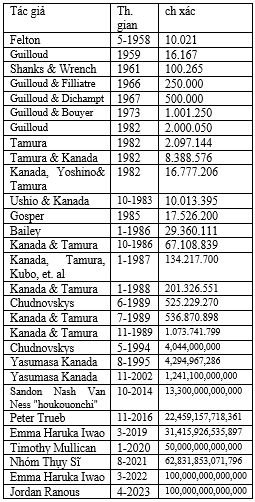
\includegraphics[width= 1\linewidth]{5}
%		\caption{\small\textit{\color{}}}
		\vspace*{-10pt}
	\end{figure}
%	\begin{tabular}{|l|c|c|l|}
%		\hline
%		Tác giả& 	Th. gian&	ch xác
%		Felton	5-1958	10.021
%		Guilloud	1959	16.167
%		Shanks & Wrench	1961	100.265
%		Guilloud & Filliatre	1966	250.000
%		Guilloud & Dichampt	1967	500.000
%		Guilloud & Bouyer	1973	1.001.250
%		Guilloud	1982	2.000.050
%		Tamura	1982	2.097.144
%		Tamura & Kanada	1982	8.388.576
%		Kanada, Yoshino& Tamura	1982	16.777.206
%		Ushio & Kanada	10-1983	10.013.395
%		Gosper	1985	17.526.200
%		Bailey	1-1986	29.360.111
%		Kanada & Tamura	10-1986	67.108.839
%		Kanada, Tamura, Kubo, et. al	1-1987	134.217.700
%		Kanada & Tamura	1-1988	201.326.551
%		Chudnovskys	6-1989	525.229.270
%		Kanada & Tamura	7-1989	536.870.898
%		Kanada & Tamura	11-1989	1.073.741.799
%		Chudnovskys	5-1994	4,044,000,000
%		Yasumasa Kanada	8-1995	4,294,967,286
%		Yasumasa Kanada	11-2002	1,241,100,000,000
%		Sandon Nash Van Ness "houkouonchi"	10-2014	13,300,000,000,000
%		Peter Trueb	11-2016	22,459,157,718,361
%		Emma Haruka Iwao
%		3-2019	31,415,926,535,897
%		Timothy Mullican	1-2020	50,000,000,000,000
%		Nhóm Thụy Sĩ	8-2021	62,831,853,071,796
%		Emma Haruka Iwao
%		3-2022	100,000,000,000,000
%		Jordan Ranous	4-2023	100,000,000,000,000
%	\end{tabular}
	\textbf{\color{lichsutoanhoc}Phụ lục $\pmb{3}$ Thực hành tính số $\pmb{\pi}$  với GeoGebra}
	\vskip 0.1cm
	Phụ lục này giới thiệu cách tính số $\pi$ trên \textit{GeoGebra} có thể phục vụ trong dạy và học.
	\vskip 0.1cm
	\textbf{\color{lichsutoanhoc}Thuật toán tính số Pi theo chuỗi} Trong \textit{GeoGebra}, việc tính xấp xỉ số $\pi$ dựa theo các công thức dạng chuỗi là tương đối thuận tiện. Ví dụ, với công thức của Euler ($9$) cho $\frac{n^2}{6}$, ta tính tổng của chuỗi theo lệnh sau:
	\begin{align*}
		s = Sum\left( {Sequence\left( {\frac{1}{{{a^2}}},a,1,n} \right)} \right)
	\end{align*}
	với $n$ là giá trị cho trước. Ở đây lệnh \textit{Sequence} sẽ tạo ra một dãy số có các phần tử là $\frac{1}{a^2}$ với  $1 \le a \le n$. Giá trị của $\pi$  có thể được tính bằng $\sqrt{6s}$. Với giá trị $n$ càng lớn thì giá trị của $\pi$  càng chính xác hơn. Chẳng hạn, với $n = 10^6$  lệnh
	\begin{align*}
		s = Sum\left( {Sequence\left( {\frac{1}{{{a^2}}},a,1,10^6} \right)} \right)
	\end{align*}
	cho $\pi \approx 3{,}14159$ (tính toán này mất khoảng vài phút trong \textit{GeoGebra}). Các công thức khác dạng chuỗi của Euler hay của Ramanujan hoặc Comtet đều có thể tính theo phương pháp trên trong \textit{GeoGebra}.
	\vskip 0.1cm
	Với công thức Gregory -- Leibnitz hoặc các công thức dạng Machin, các số hạng của chuỗi liên quan đến các số lẻ và dấu được đảo liên tiếp. Biểu thức tính dấu của mỗi số hạng sẽ tương đối phức tạp. Tuy nhiên, ta có thể sử dụng mẹo đặt bước của dãy số là $4$ và sinh hai thay vì chỉ một số hạng ở mỗi bước. Ví dụ với công thức Gregory--Leibnitz ta làm như sau:
	\begin{align*}
		4*Sum\!\!\left(\!\! {Sequence\left(\!\! {\frac{1}{a}\! -\! \frac{1}{{a \!+\! 2}},a,1,n \!+\! 1,4} \!\!\right)}\!\! \right)
	\end{align*}
	với $n$ là một số chia hết cho $4$. Các số hạng sẽ được sinh theo cặp:$1 - \frac{1}{3}, \frac{1}{5} - \frac{1}{7}, \ldots$.
	\vskip 0.1cm  
	Với  $n = 10^6$, ta thu được giá trị của $\pi$  là $3{,}14159$. Bạn đọc có thể tự sử dụng cách này để tính  $\pi$  theo các công thức dạng Machin.
	\vskip 0.1cm
	\textbf{\color{lichsutoanhoc}Tính số Pi trên GeoGebra theo Archimedes}
	\vskip 0.1cm 
	Có thể sử dụng \textit{GeoGebra} để minh họa cách tính số $\pi$  theo thuật toán Archimedes như sau. Thiết lập các đường tròn cùng với các đa giác đều nội ngoại tiếp theo các bước sau. Cũng có thể sử dụng các file .ggb \textit{GeoGebra} có sẵn trên mạng.  
	\vskip 0.1cm
	\textbf{\color{lichsutoanhoc}Bước} $\pmb1$: Dùng công cụ vẽ đường tròn 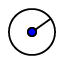
\includegraphics[scale =0.25]{6}: Khai báo tâm (nhấn chuột được một điểm), chọn bán kính $0.5$ (đường kính bằng $1$).
	\vskip 0.1cm 
	\textbf{\color{lichsutoanhoc}Bước} $\pmb{2}$: Phóng to hình cho dễ nhìn đường tròn.
	\vskip 0.1cm
	\textbf{\color{lichsutoanhoc}Bước} $\pmb{3}$: Vẽ đa giác đều nhớ công cụ 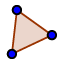
\includegraphics[scale =0.25]{7} đa giác đều (thí dụ, tam giác hoặc tứ giác đều). Nháy vào đỉnh đầu tiên để kết thúc vẽ đa giác đều nội tiếp.
	\vskip 0.1cm
	\textbf{\color{lichsutoanhoc}Bước} $\pmb{4}$: Chọn nút công cụ chuyển động 
\includegraphics[scale =0.25]{8} và vẫn giữ nguyên hình (tam giác hoặc vuông).
	\vskip 0.1cm
	\textbf{\color{lichsutoanhoc}Bước} $\pmb{5}$: Chọn công cụ Khoảng cách hoặc Độ dài.  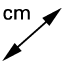
\includegraphics[scale =0.25]{9}. Chọn một điểm bên trong đường tròn nội tiếp để xuất hiện số đo chu vi. Ghi số đo chu vi xuống phía dưới. 
	\vskip 0.1cm
	\textbf{\color{lichsutoanhoc}Bước} $\pmb{6}$: Dùng quy trình trên để vẽ và tìm chu vi đa giác đều $6$ cạnh, $12$ cạnh, $24$, $48$ và $96$ cạnh.
	\vskip 0.1cm
	\textbf{\color{lichsutoanhoc}Bước} $\pmb{7}$: Làm tương tự với đa giác đều ngoại tiếp và so sánh với chu vi đa giác đều nội tiếp và đi đến kết luận xấp xỉ số $\pi$.
	\vskip 0.1cm  
	Dưới đây là một số hình ảnh minh họa. :
	\begin{figure}[H]
		\vspace*{-5pt}
		\centering
		\captionsetup{labelformat= empty, justification=centering}
		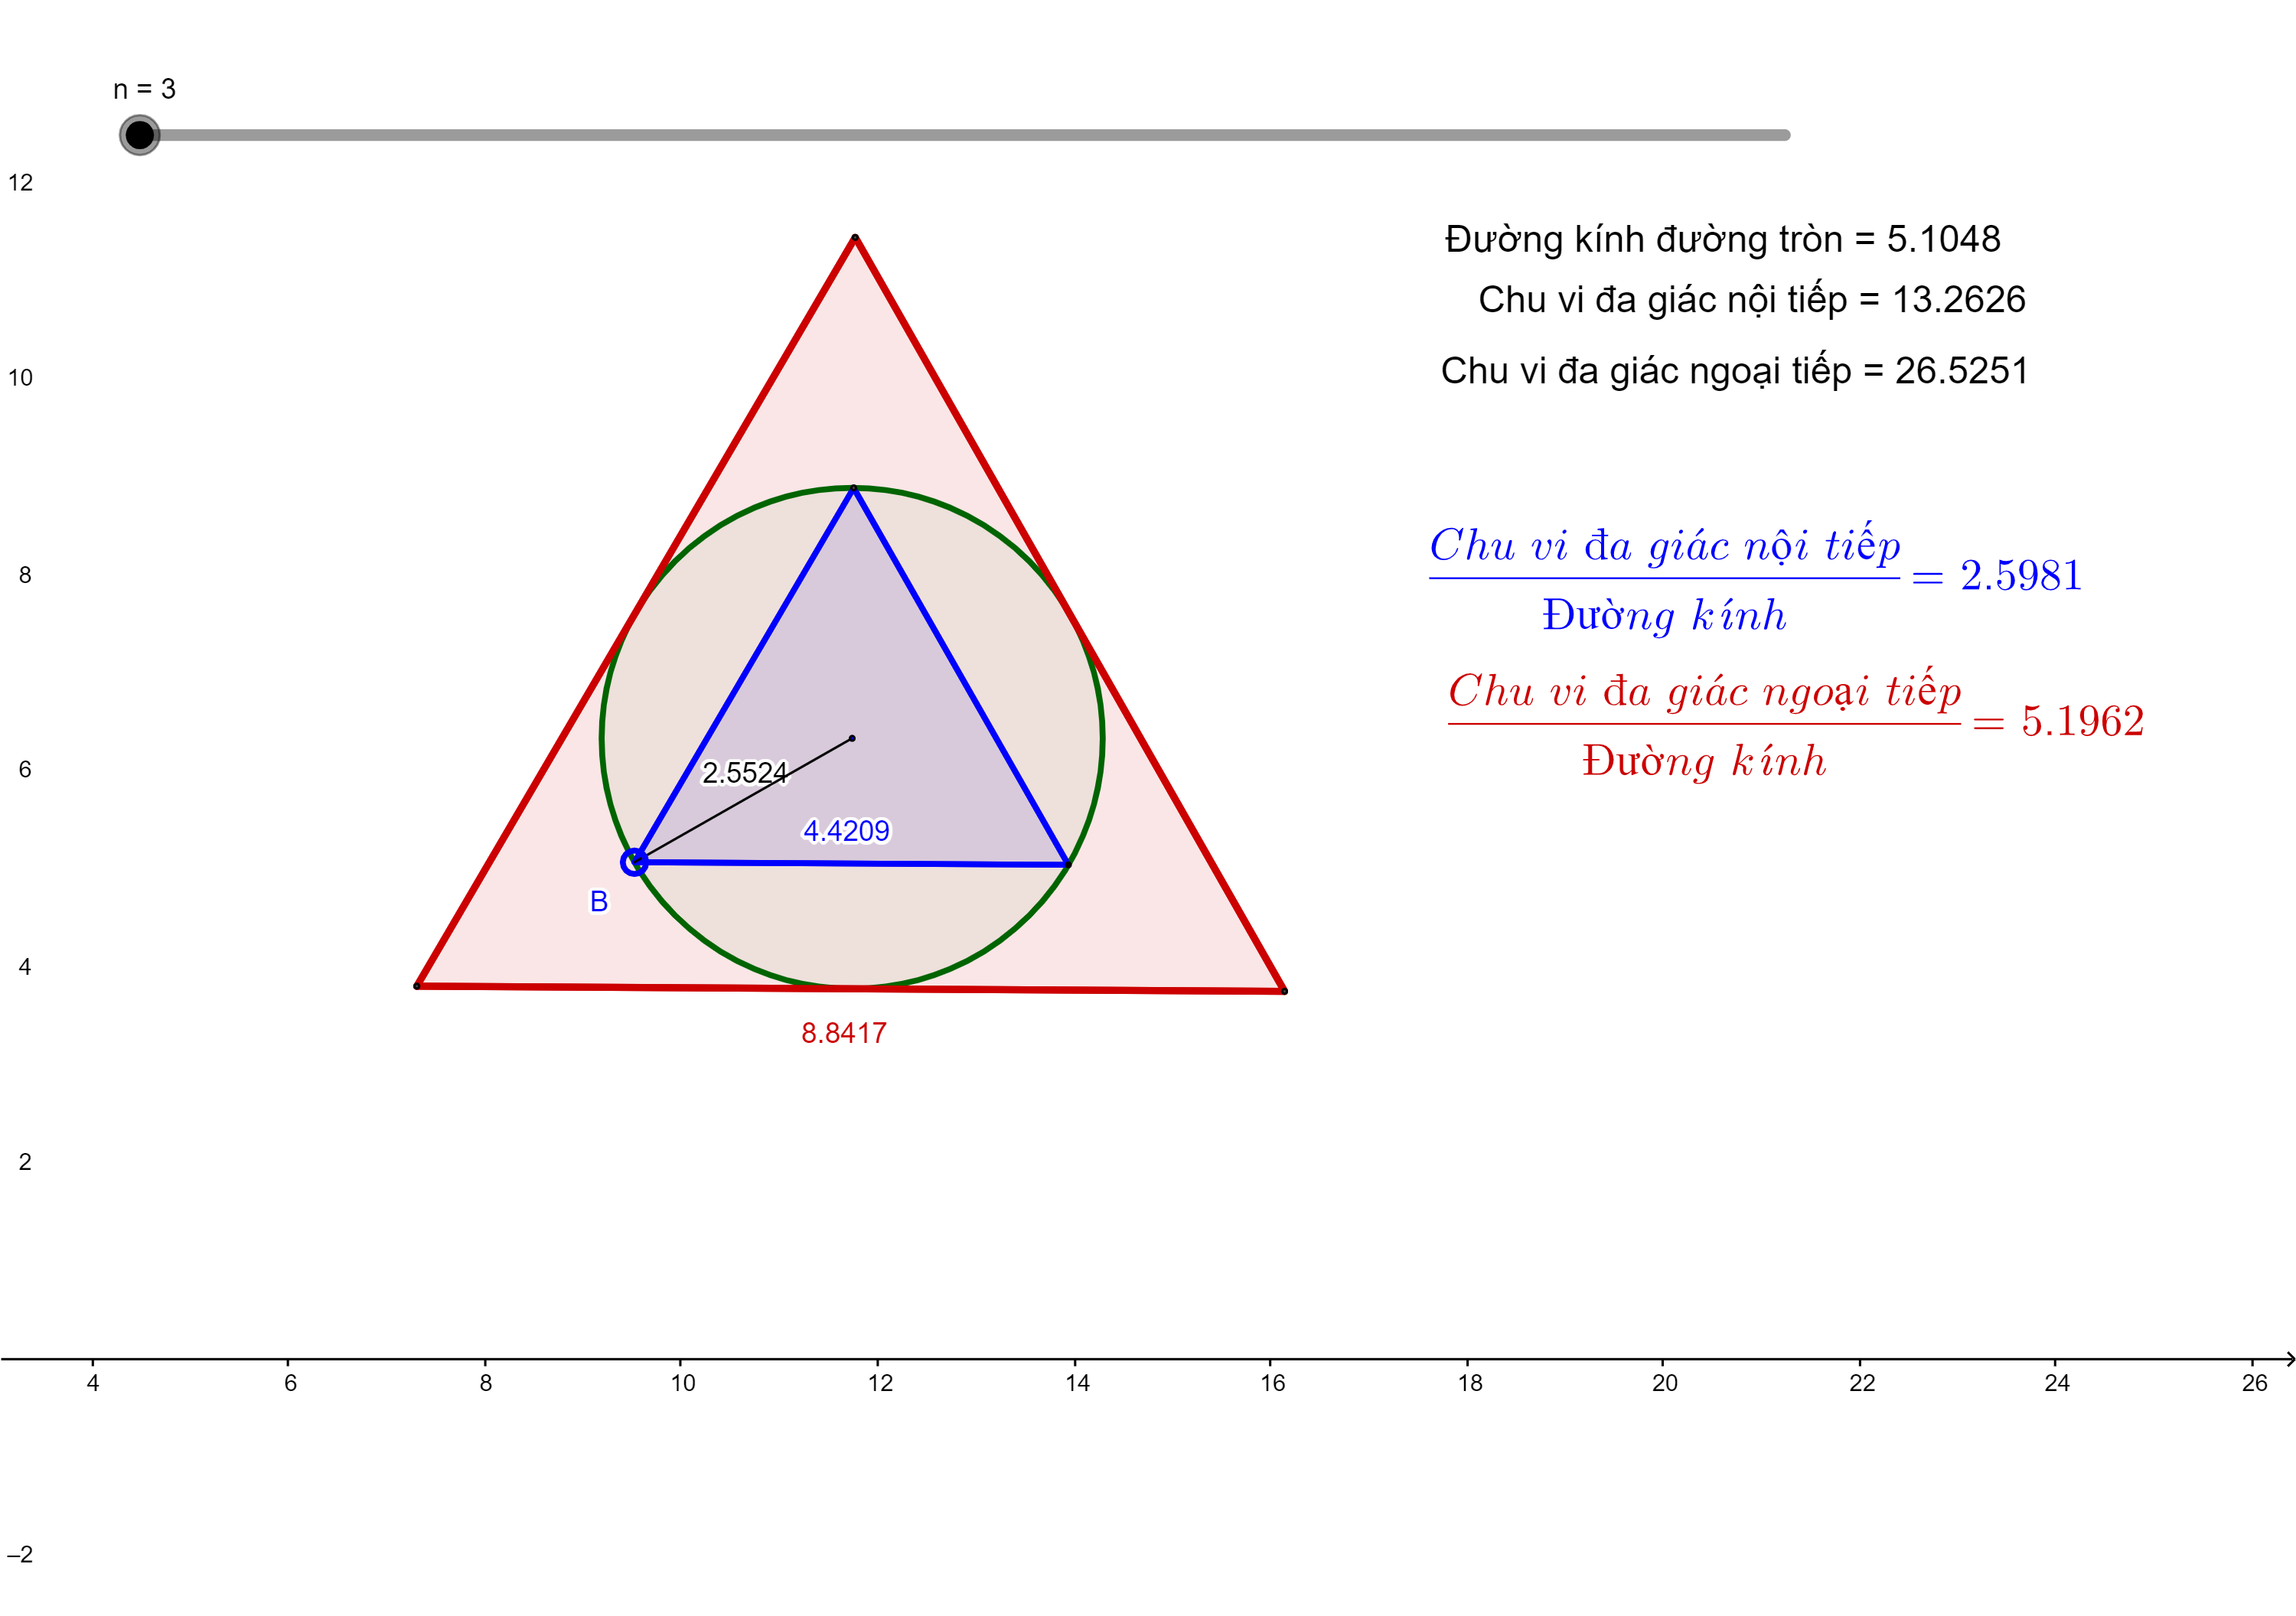
\includegraphics[width= 1\linewidth]{10}
		\caption{\small\textit{\color{lichsutoanhoc}$n = 3$}}
		\vspace*{-10pt}
	\end{figure}
	\begin{figure}[H]
		\vspace*{-5pt}
		\centering
		\captionsetup{labelformat= empty, justification=centering}
		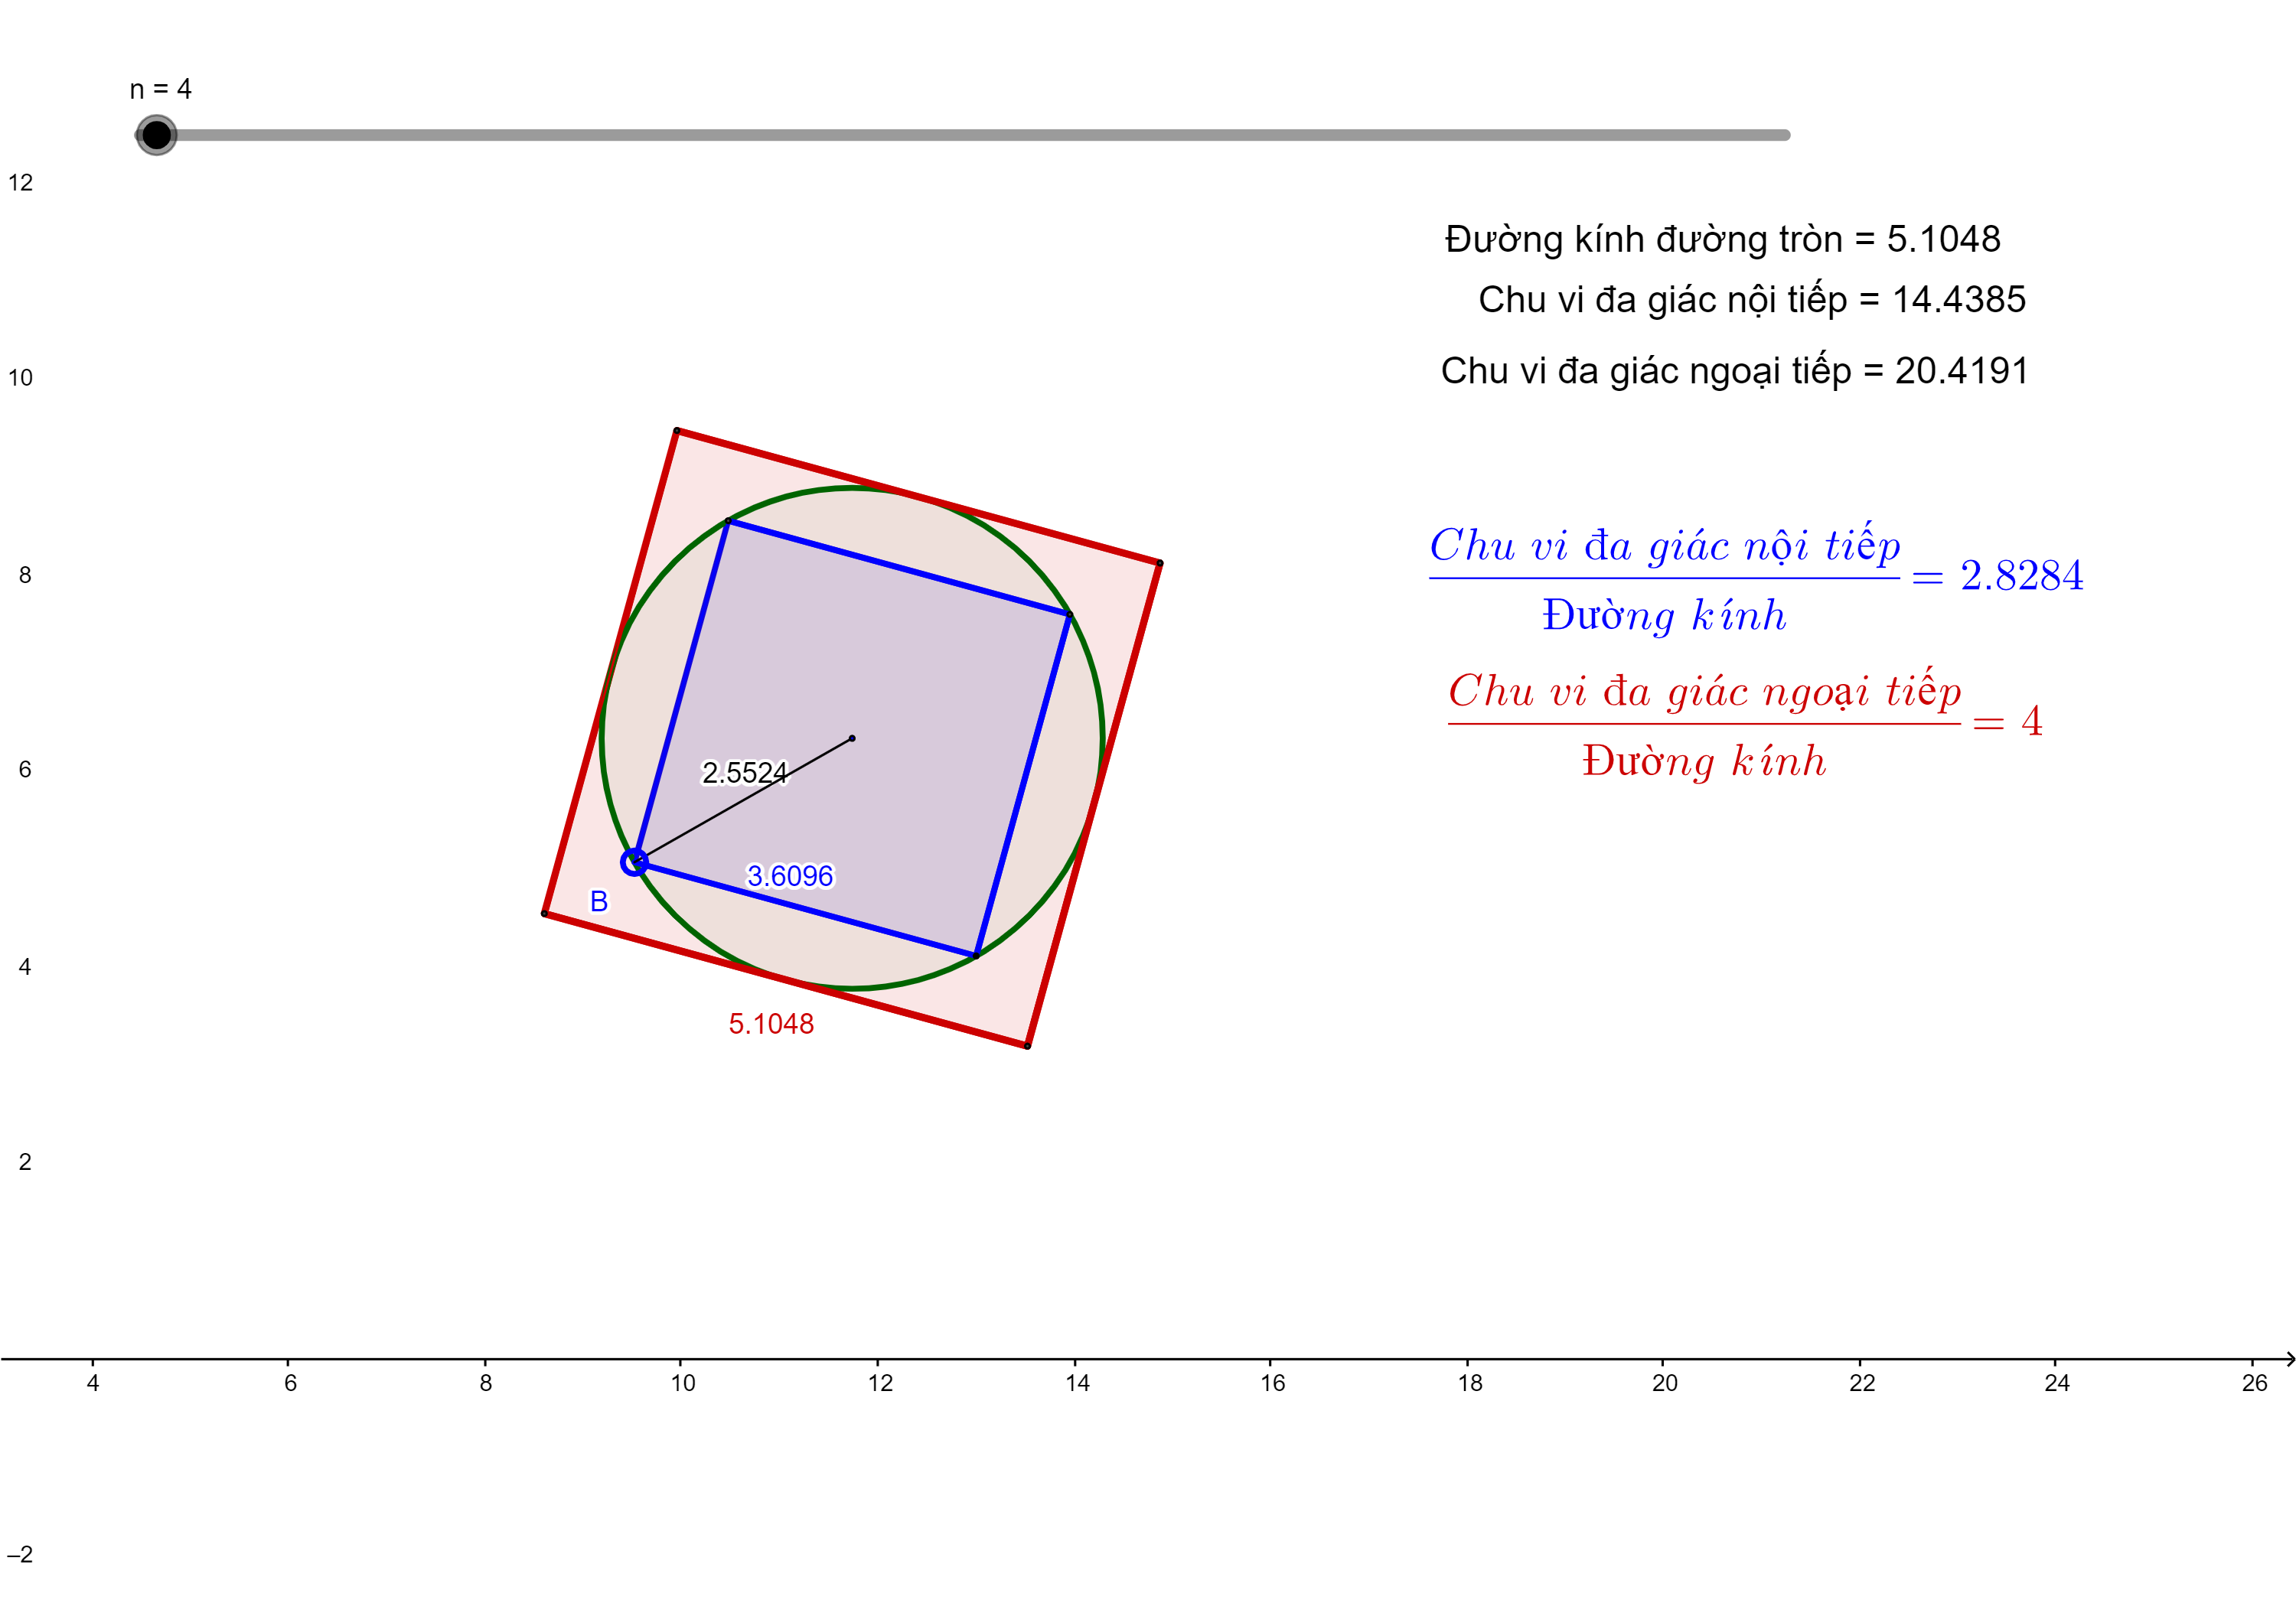
\includegraphics[width= 1\linewidth]{11}
	\caption{\small\textit{\color{lichsutoanhoc}$n = 4$.}}
	\end{figure}
%	\begin{figure}[H]
%		\vspace*{-5pt}
%		\centering
%		\captionsetup{labelformat= empty, justification=centering}
%		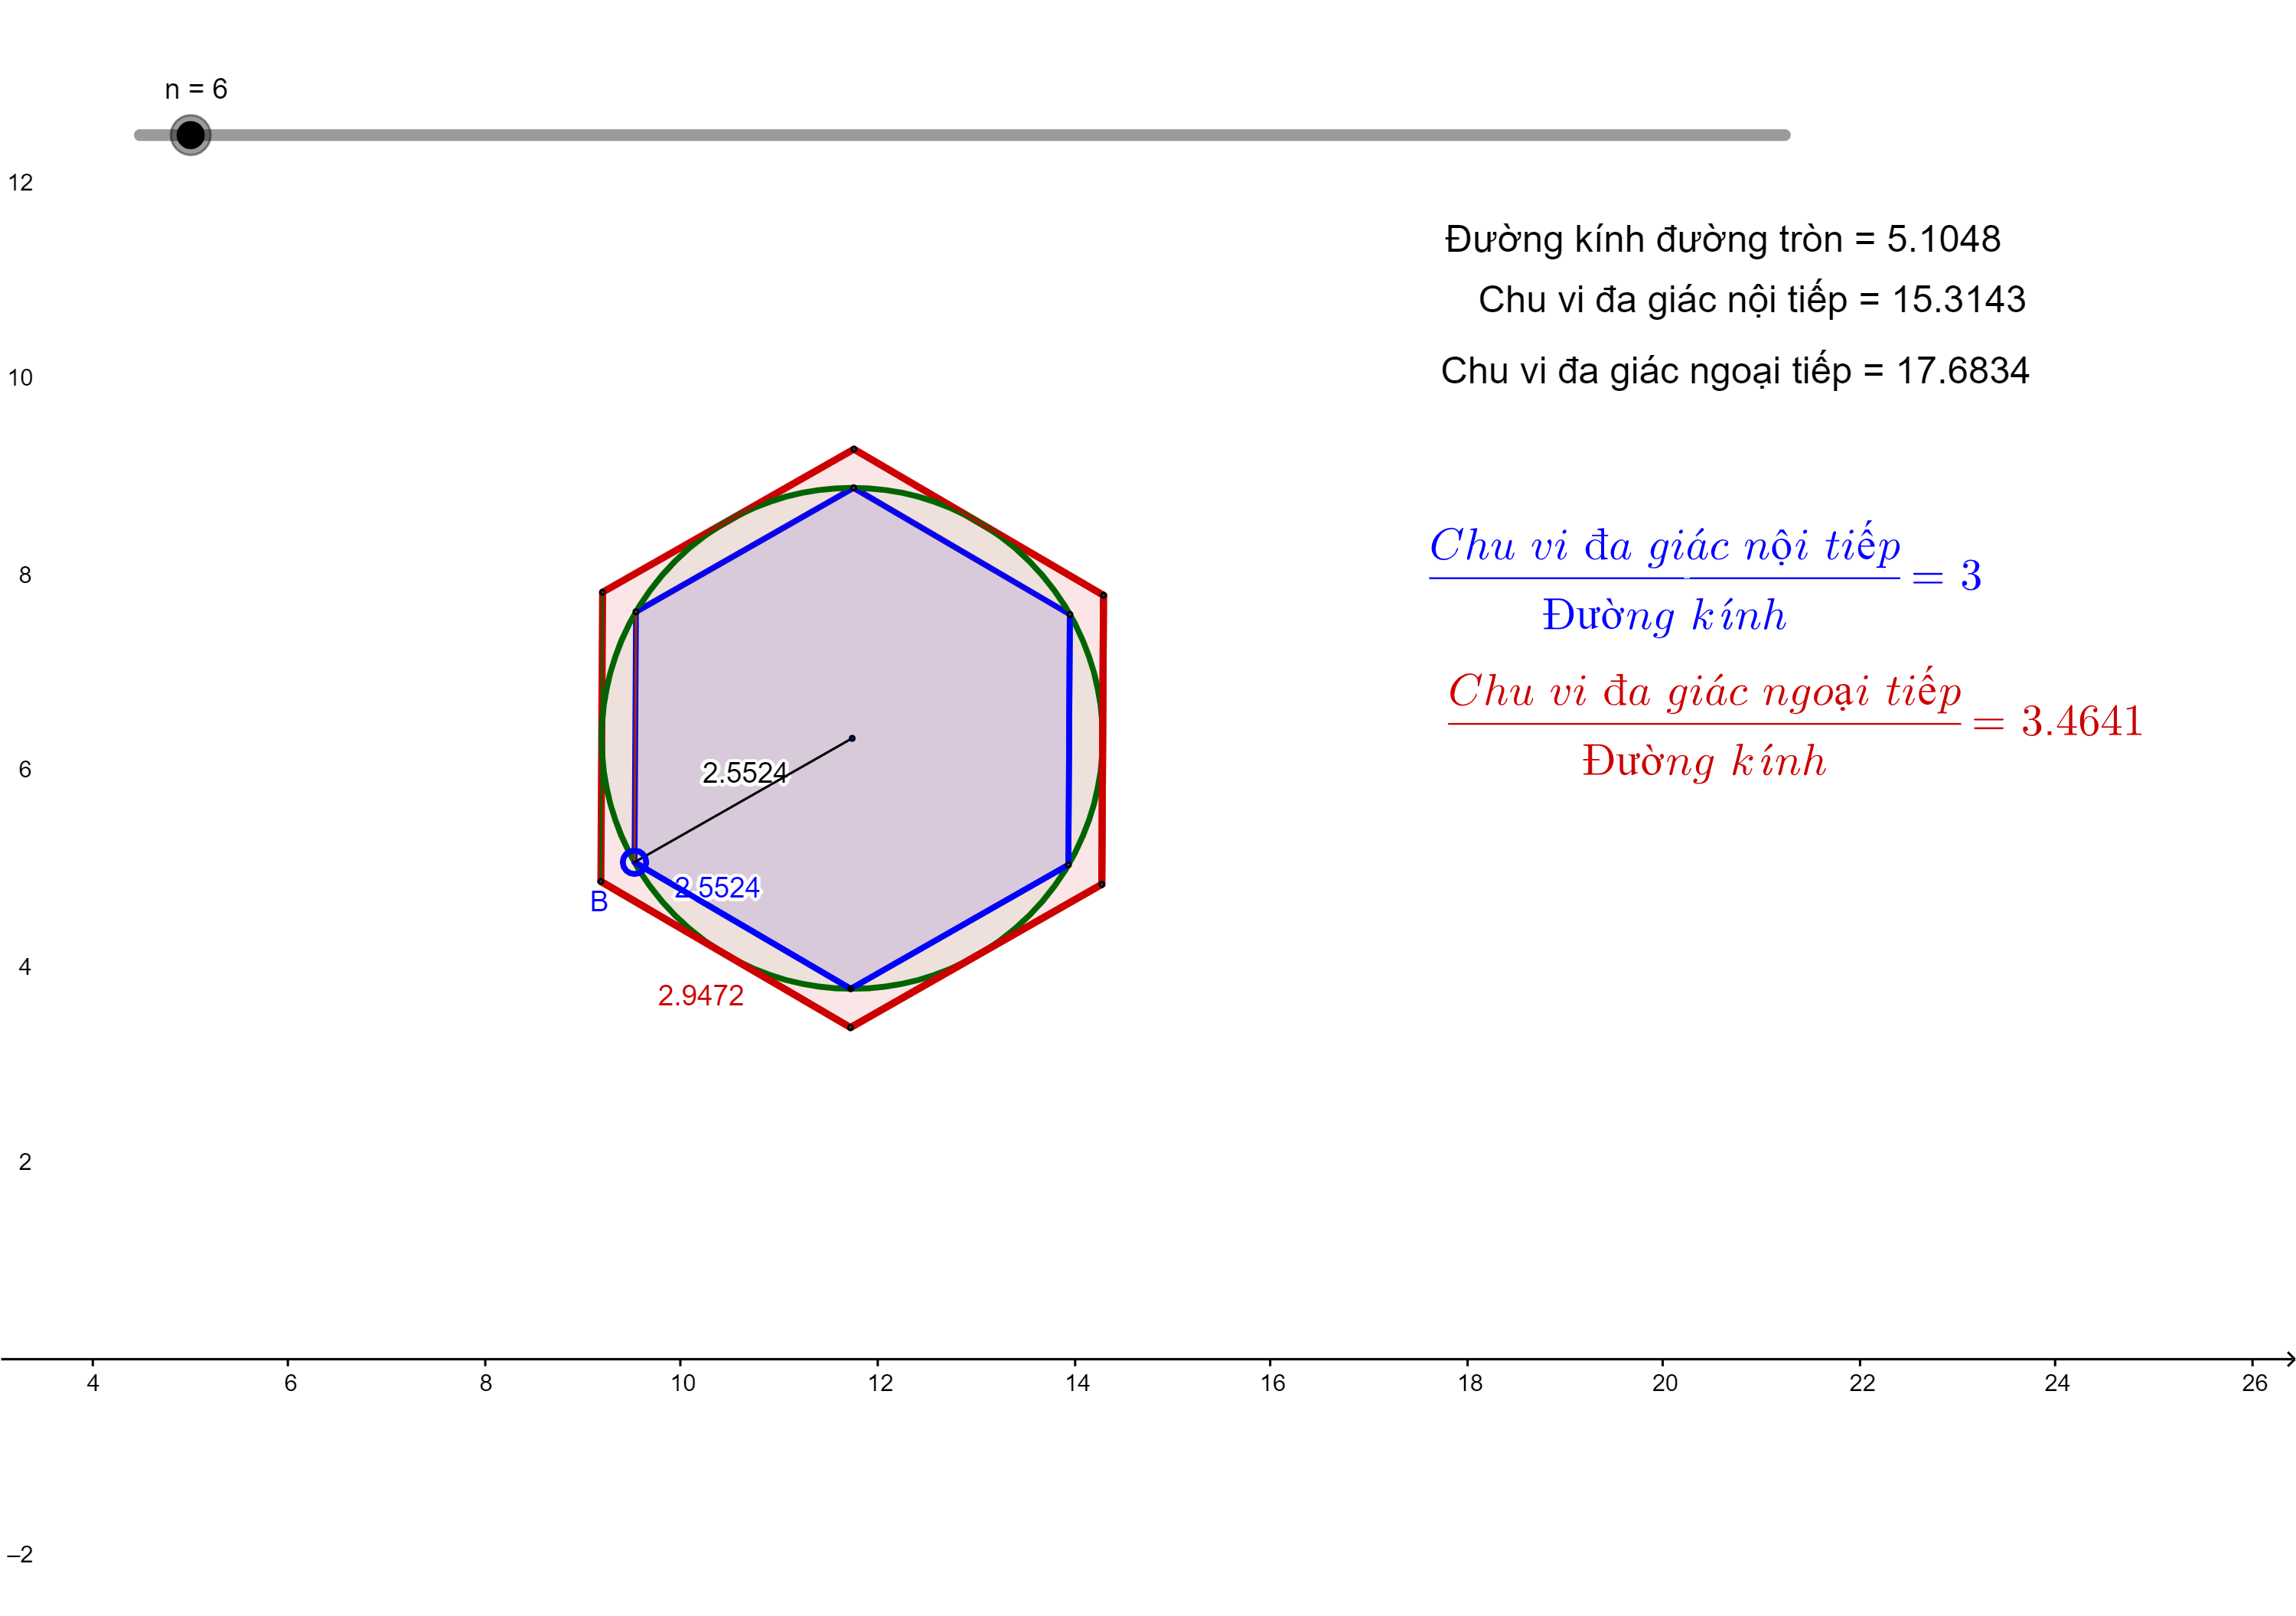
\includegraphics[width= 1\linewidth]{12}
%		\caption{\small\textit{\color{lichsutoanhoc}$n = 6$.}}
%		\vspace*{-10pt}
%	\end{figure}
	\begin{figure}[H]
		\vspace*{-5pt}
		\centering
		\captionsetup{labelformat= empty, justification=centering}
		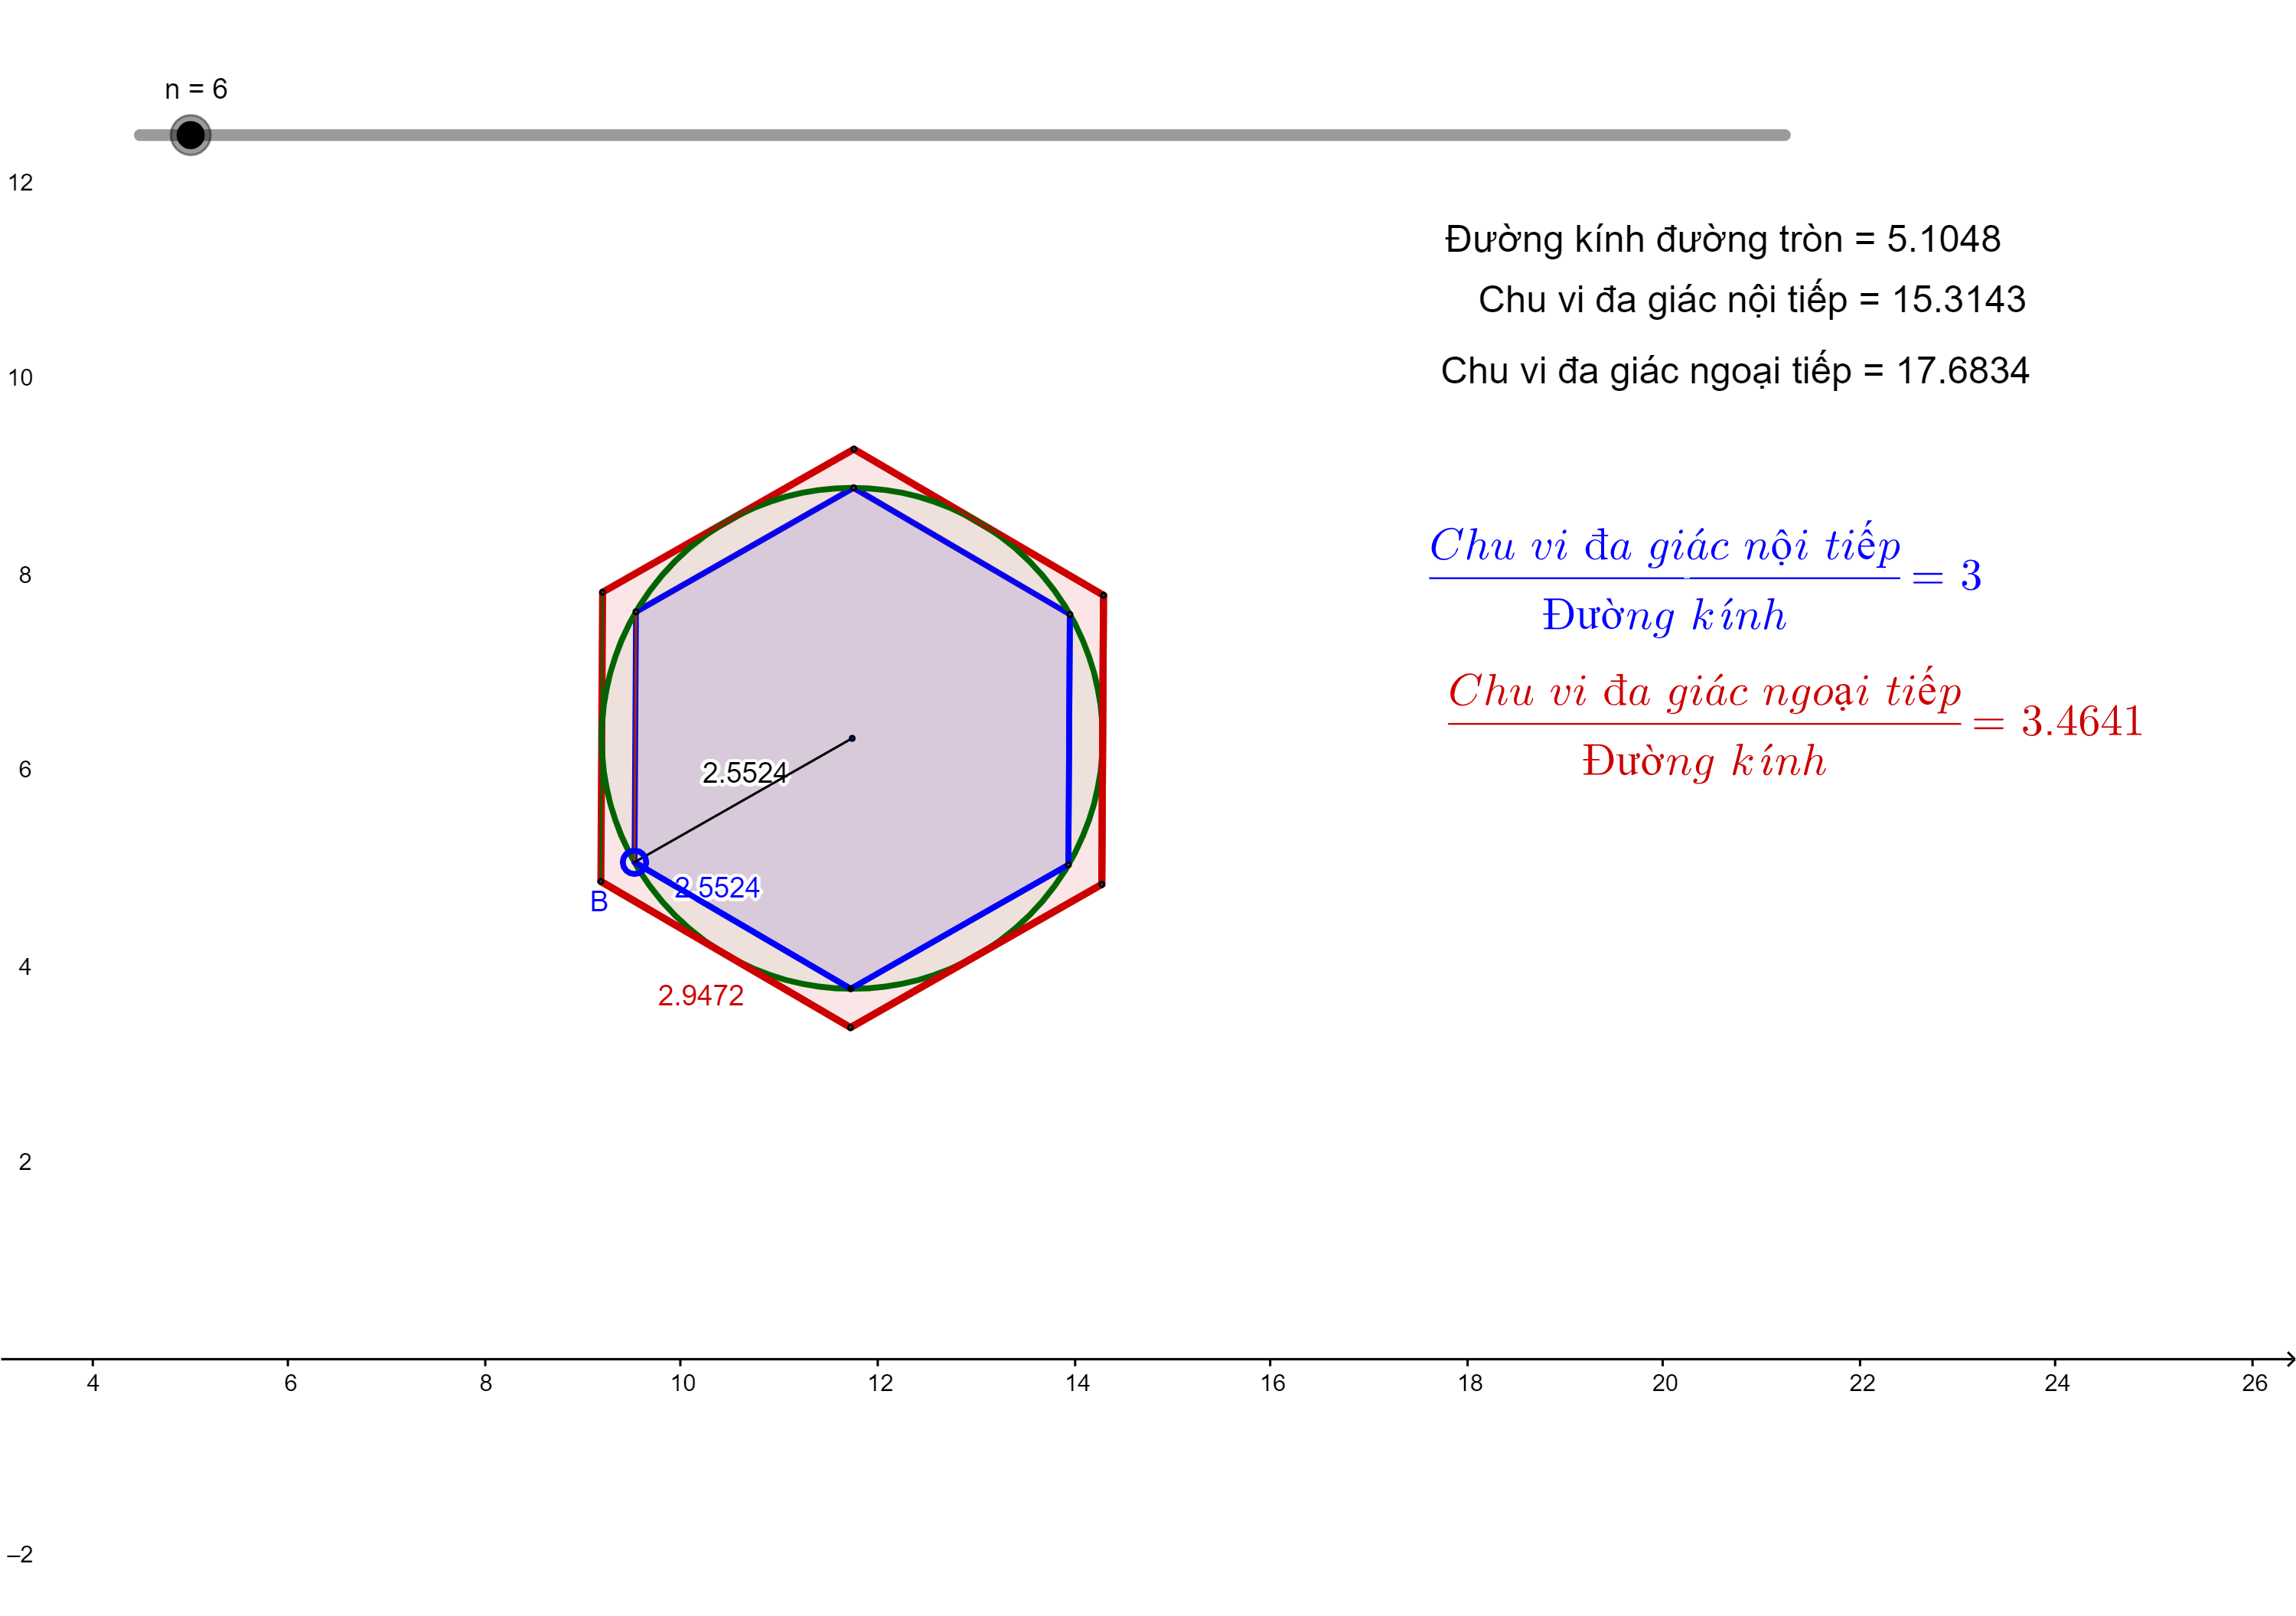
\includegraphics[width= 1\linewidth]{12}
		\caption{\small\textit{\color{lichsutoanhoc}$n = 6$.}}
		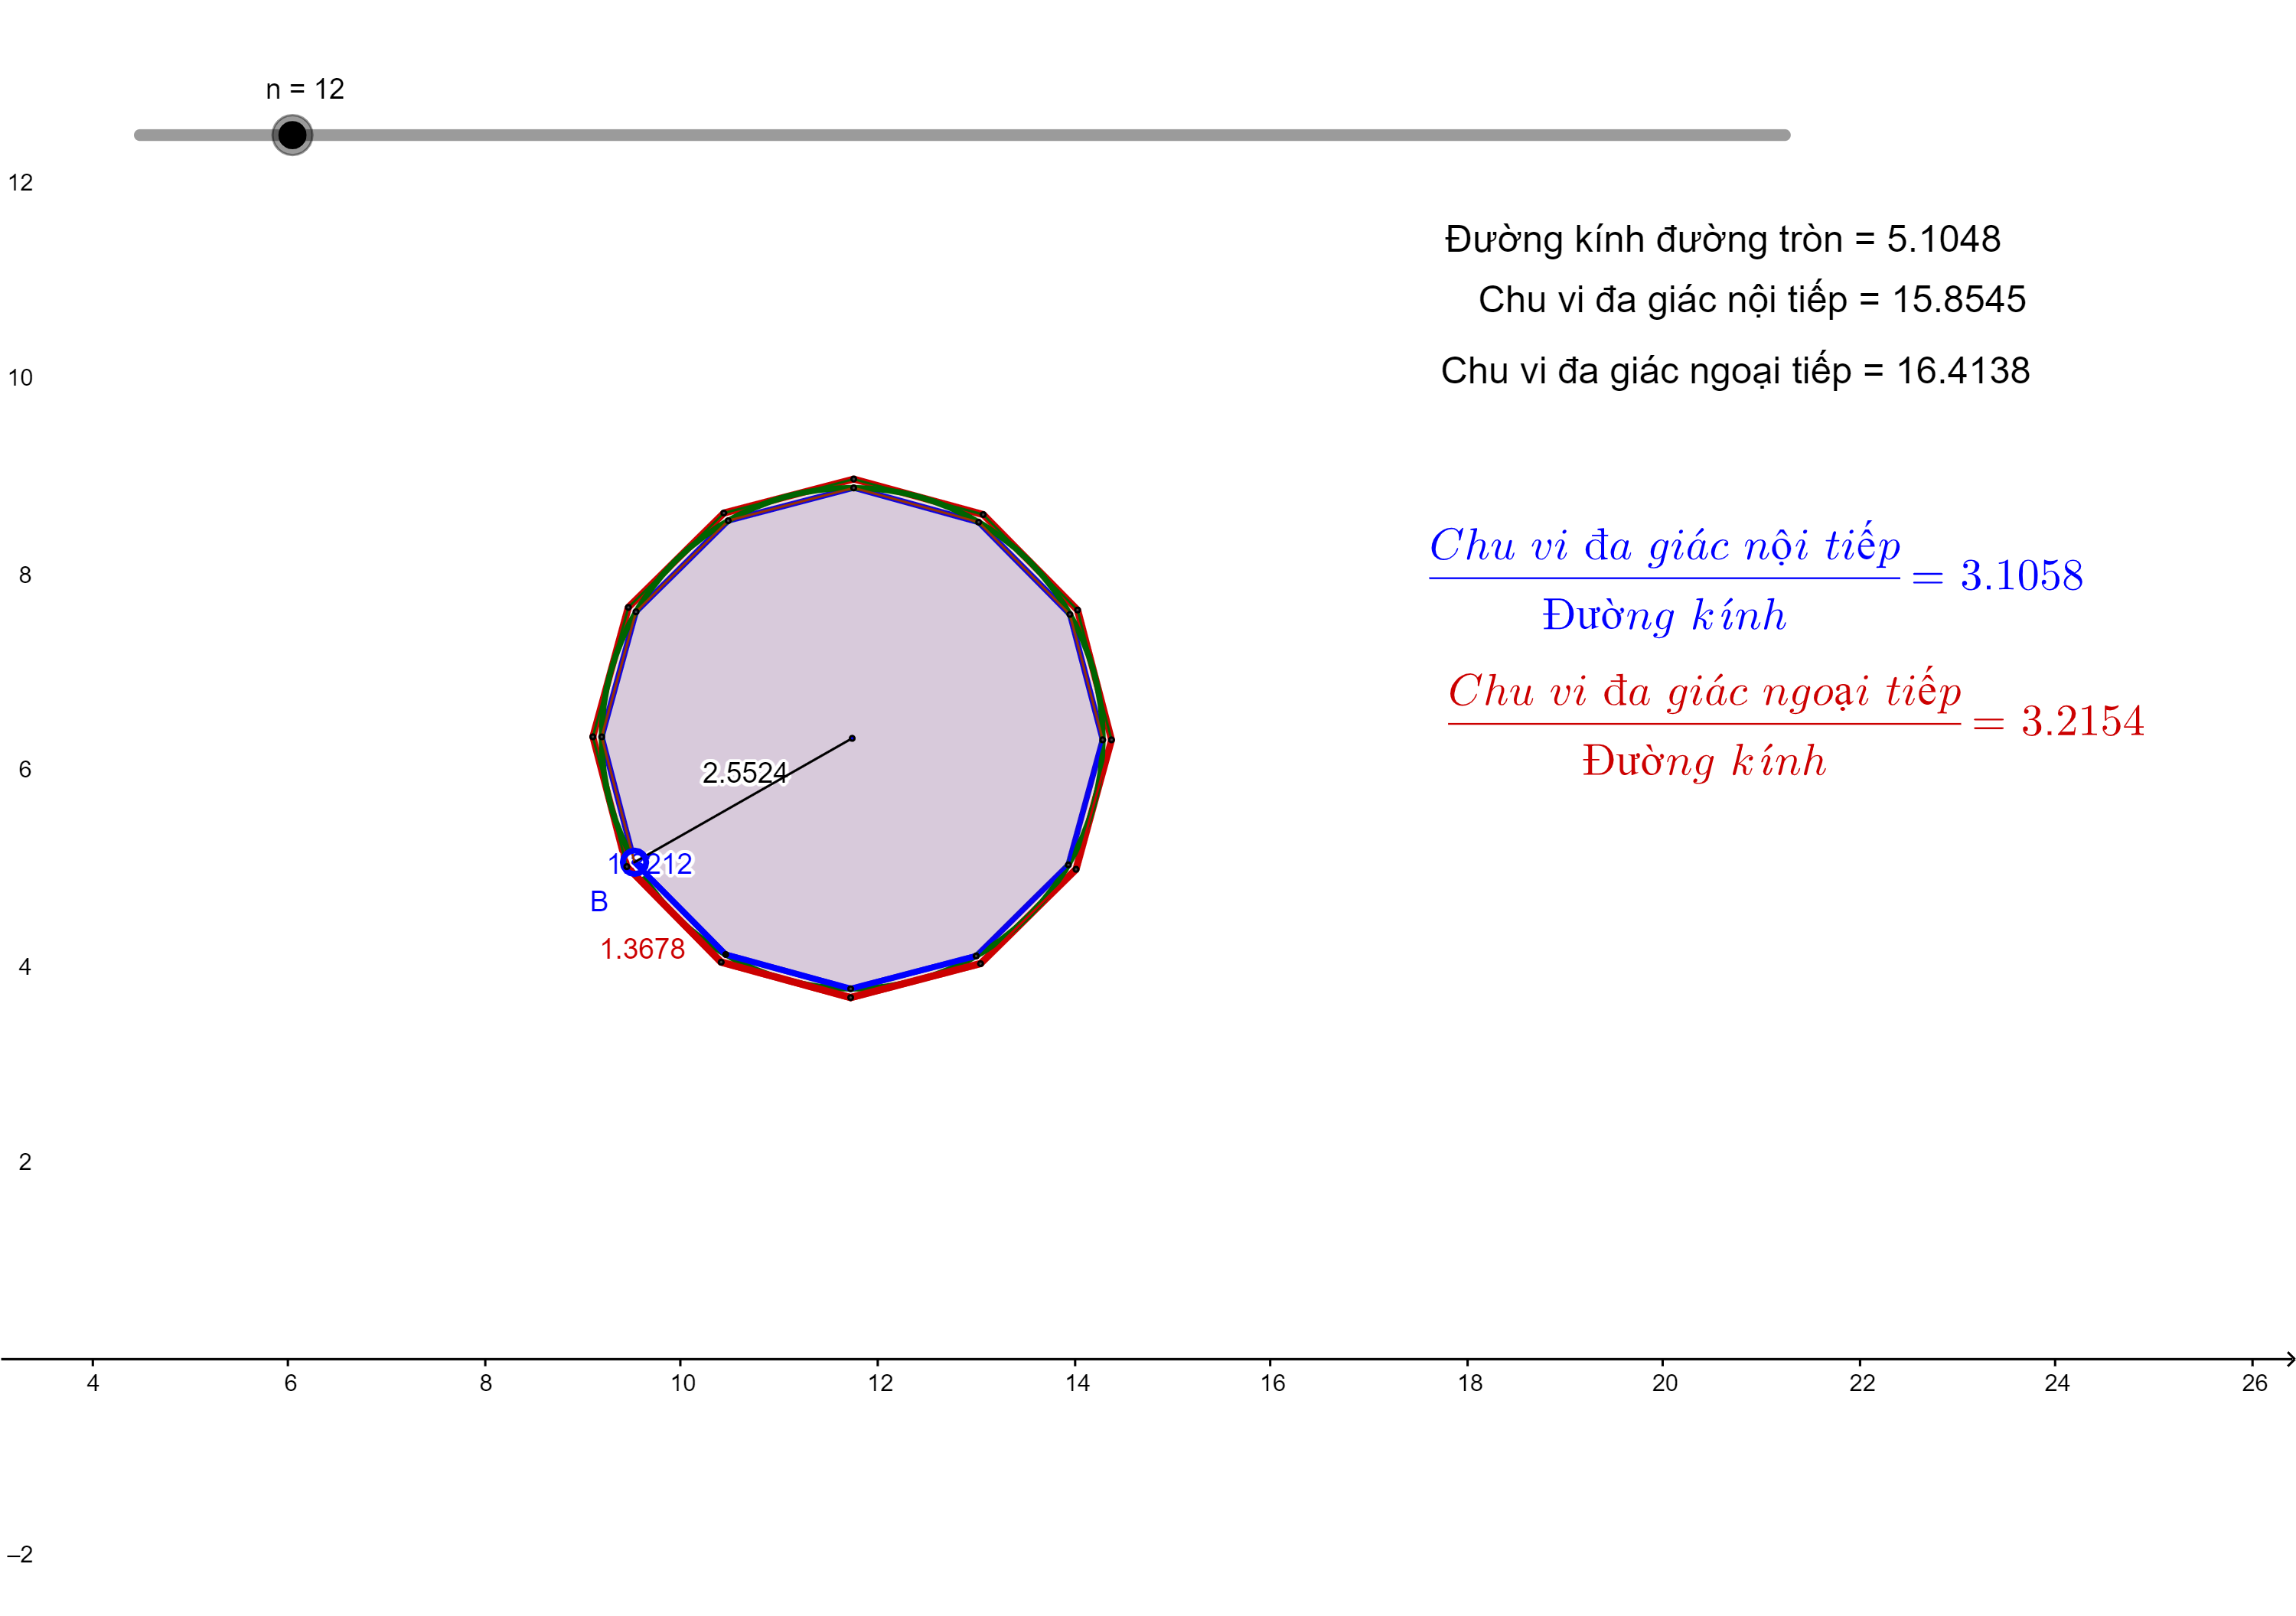
\includegraphics[width= 1\linewidth]{13}
		\caption{\small\textit{\color{lichsutoanhoc}$n = 12$.}}
		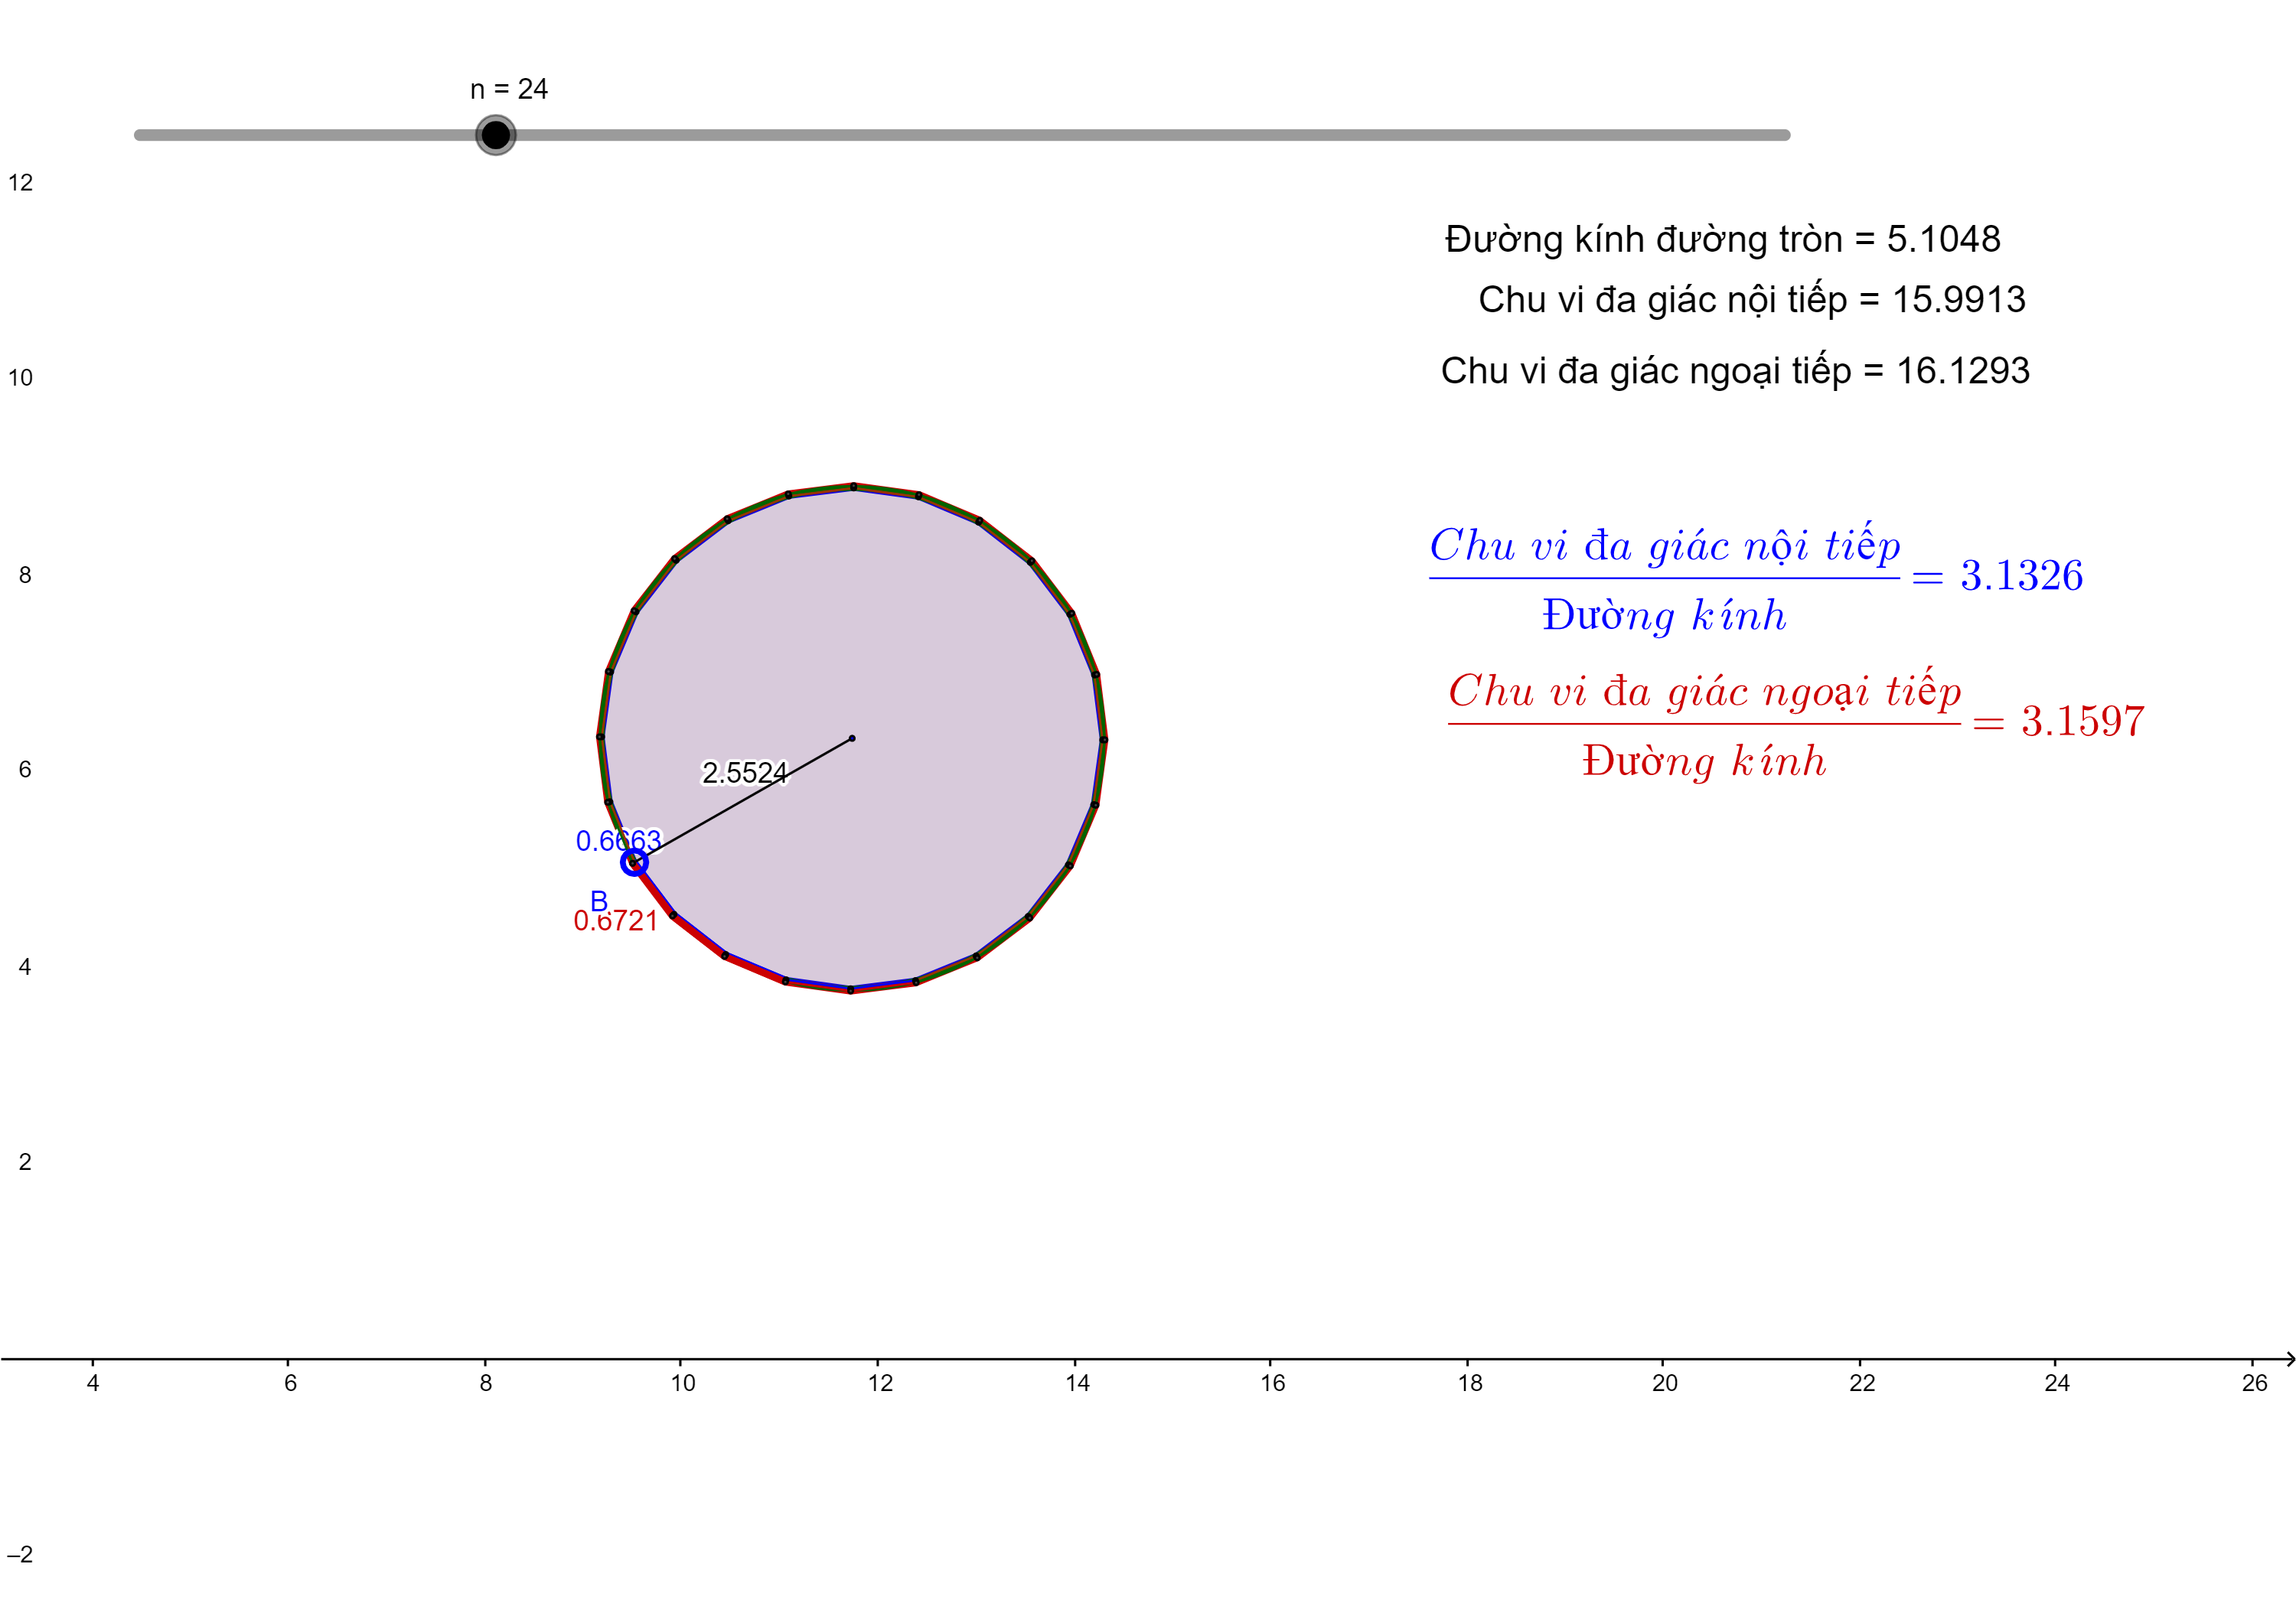
\includegraphics[width= 1\linewidth]{14}
		\caption{\small\textit{\color{lichsutoanhoc}$n = 24$.}}
			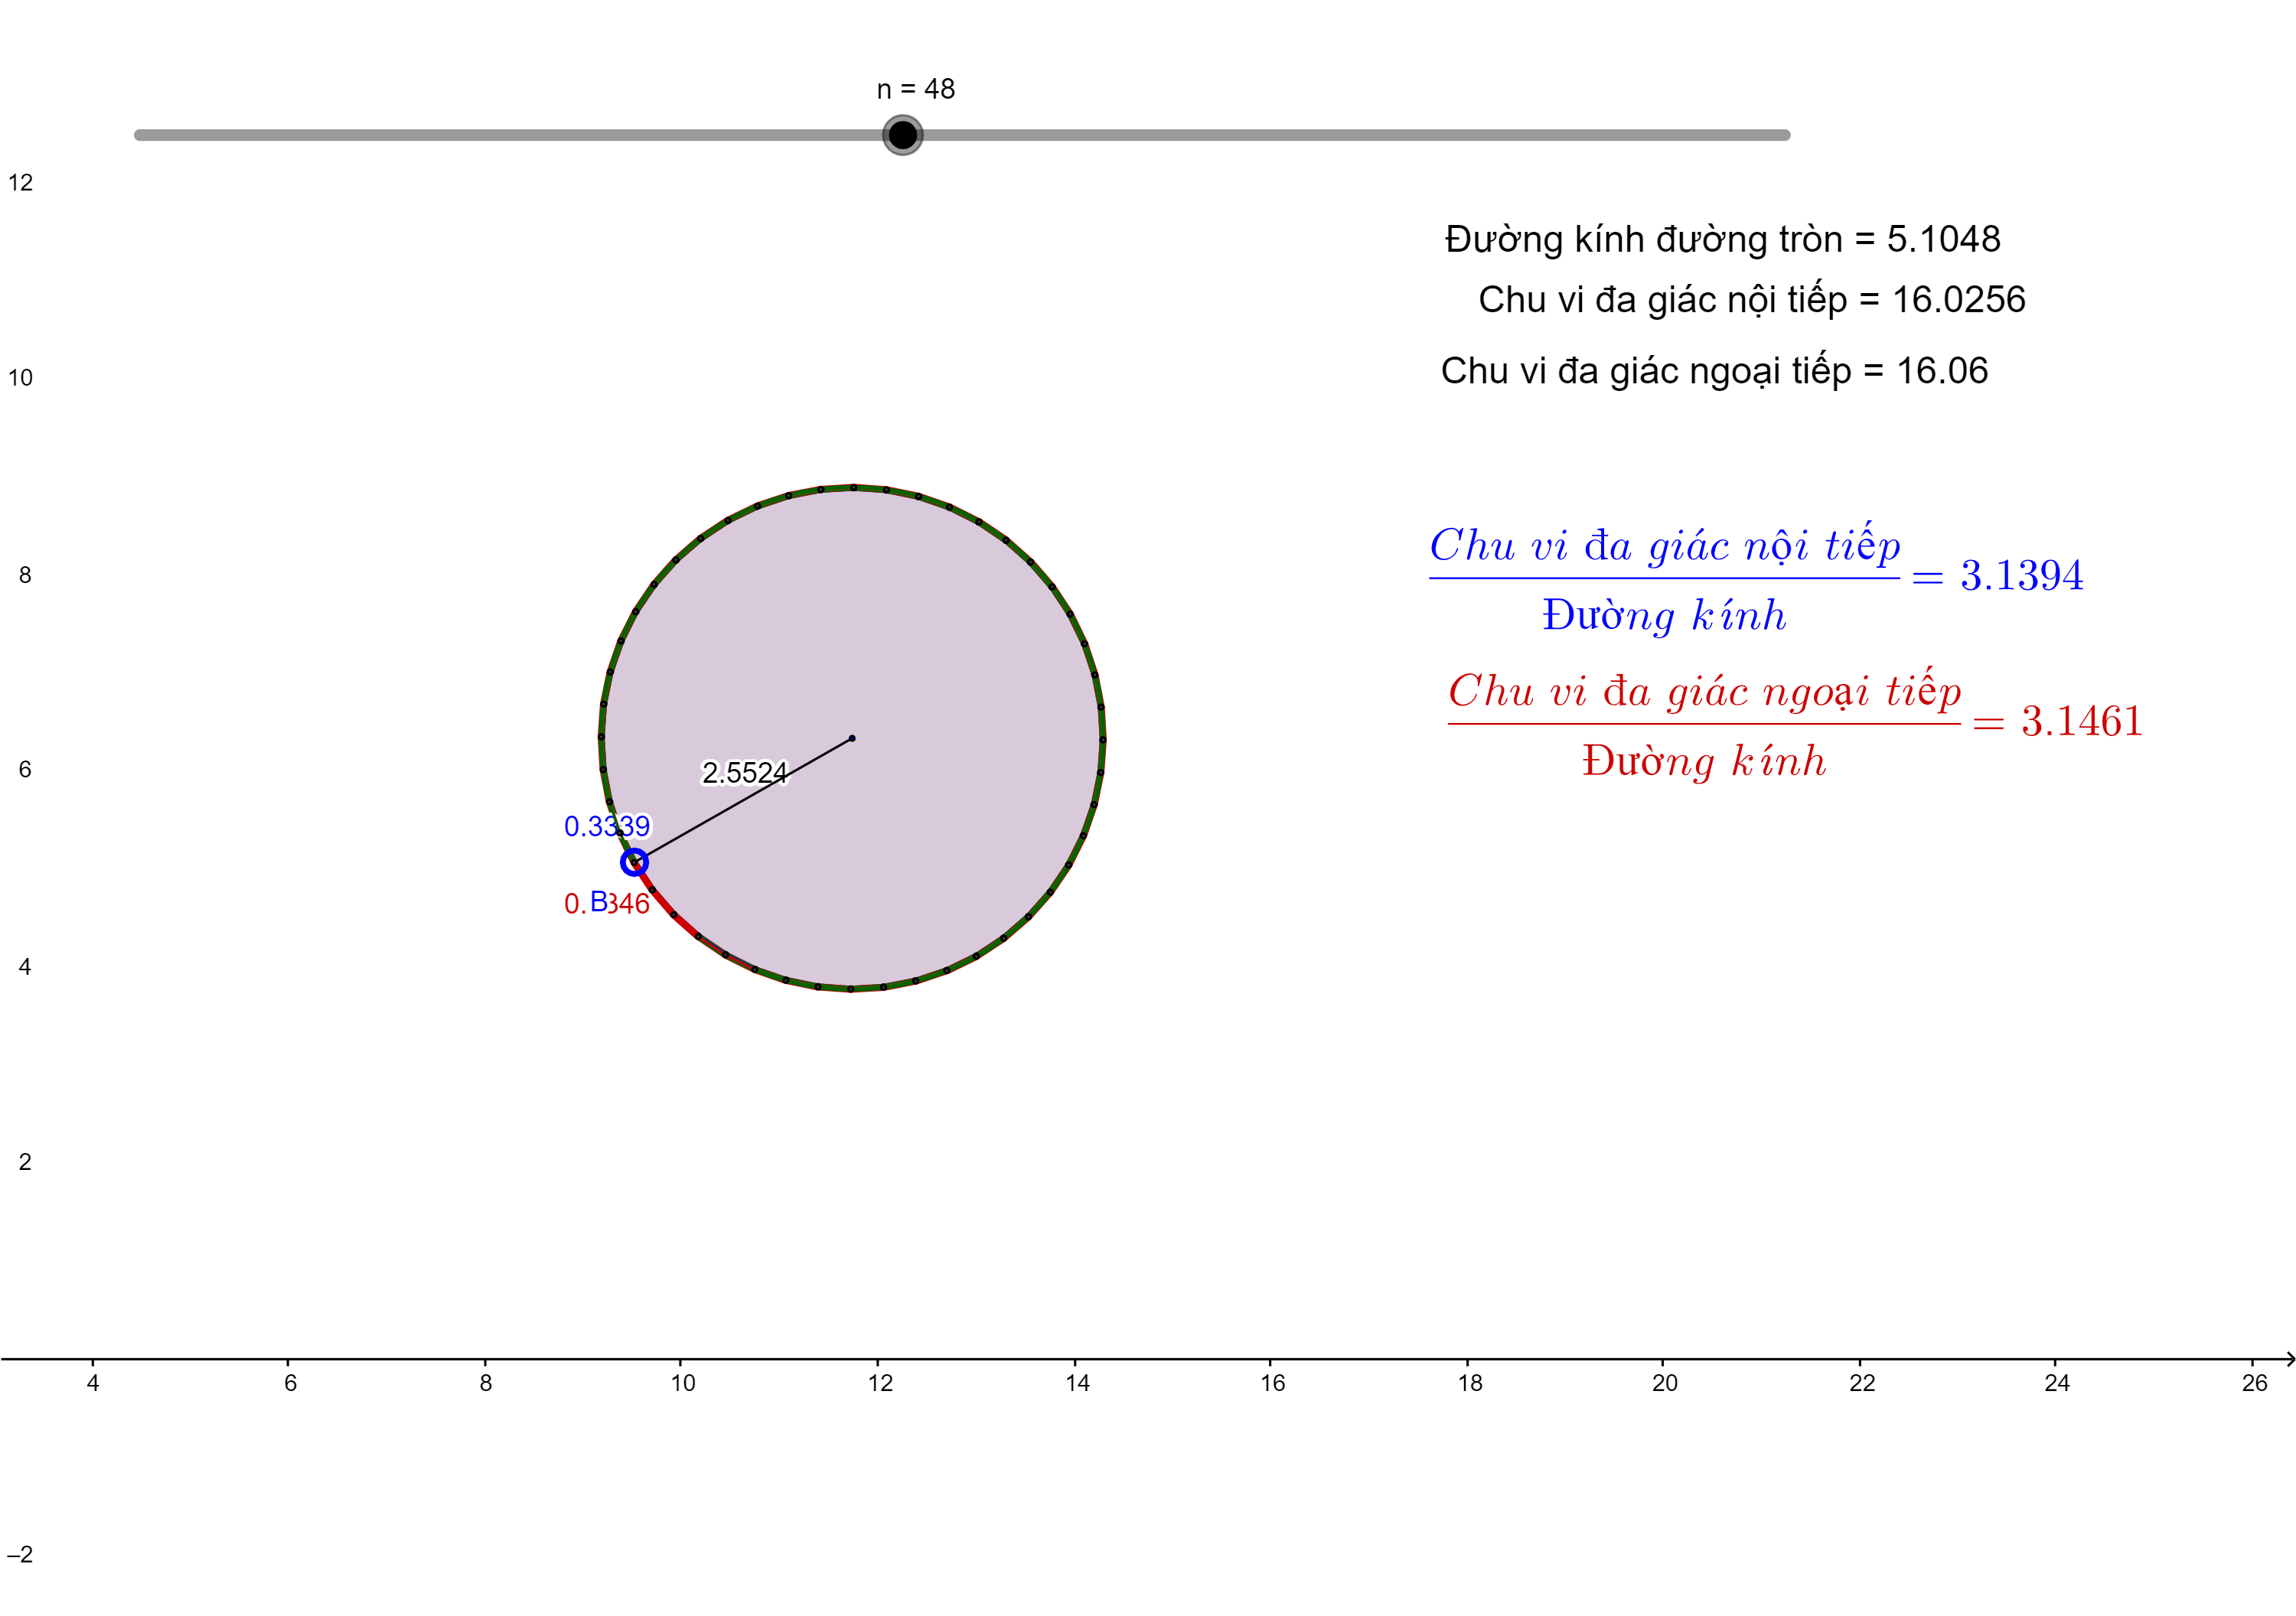
\includegraphics[width= 1\linewidth]{15}
		\caption{\small\textit{\color{lichsutoanhoc}$n = 48$.}}
		\vspace*{-10pt}
	\end{figure}
%	\begin{figure}[H]
%		\vspace*{-5pt}
%		\centering
%		\captionsetup{labelformat= empty, justification=centering}
%		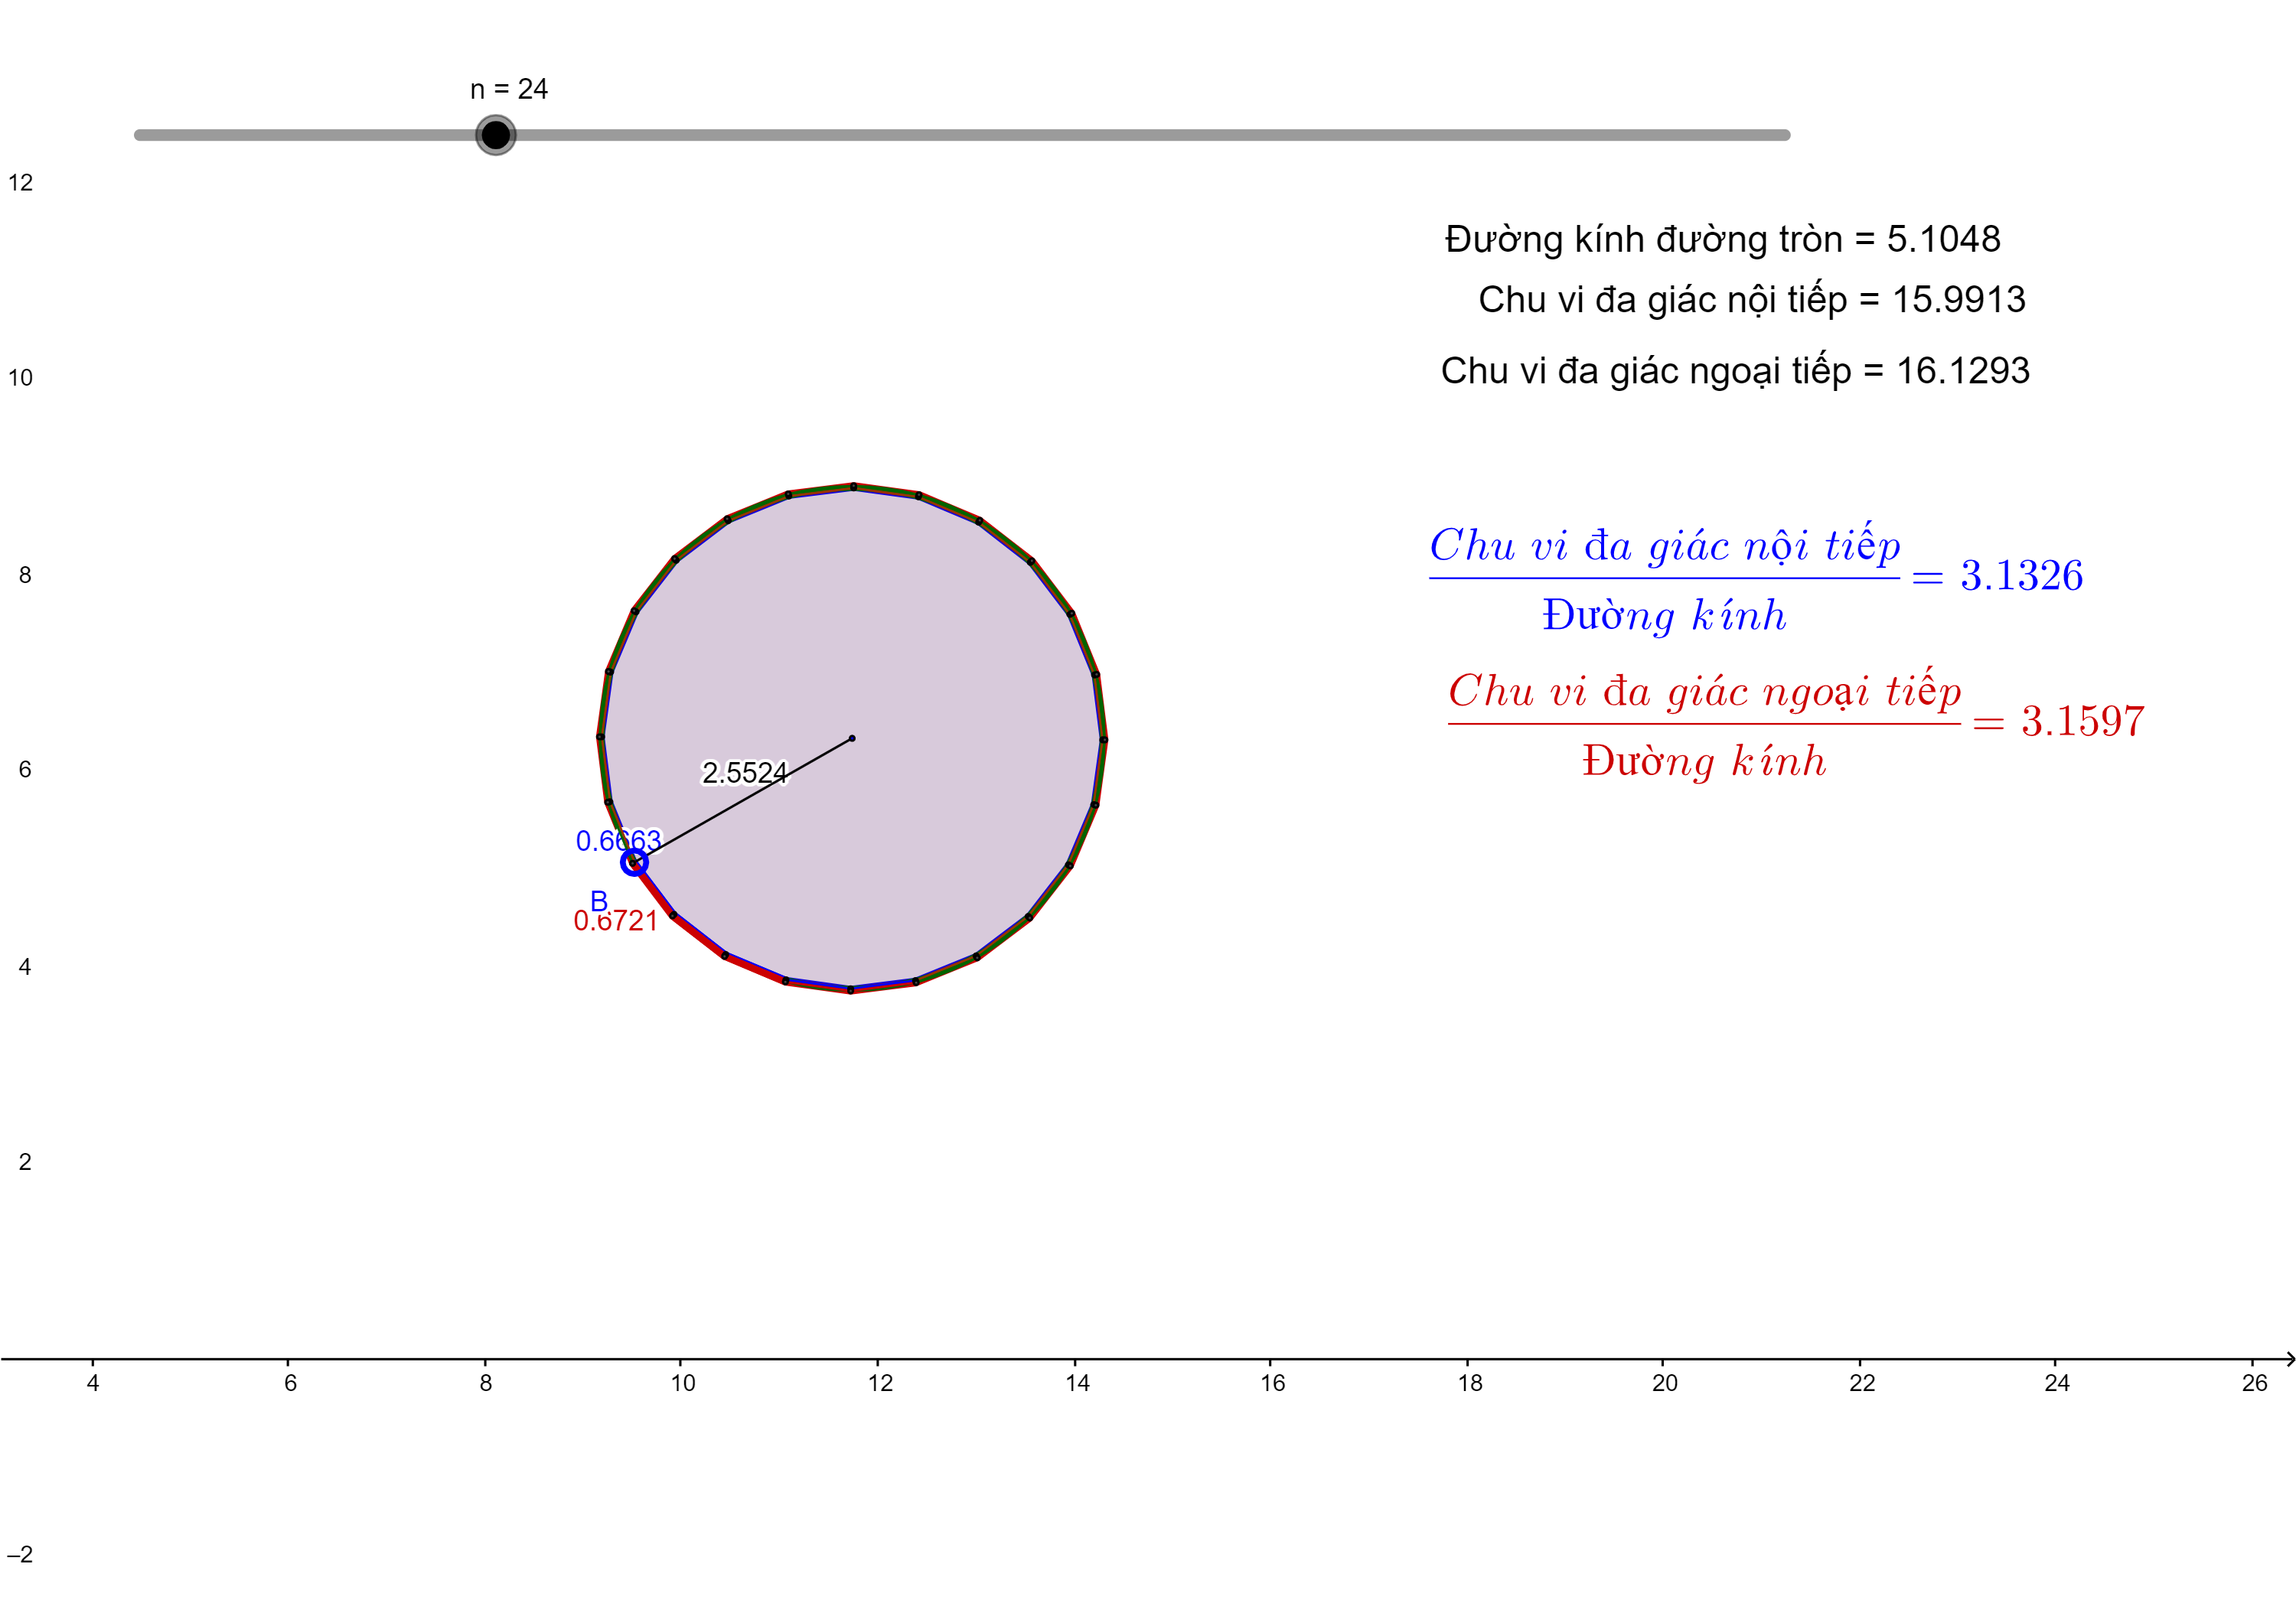
\includegraphics[width= 1\linewidth]{14}
%		\caption{\small\textit{\color{lichsutoanhoc}$n = 24$.}}
%		\vspace*{-10pt}
%	\end{figure}
%	\begin{figure}[H]
%		\vspace*{-5pt}
%		\centering
%		\captionsetup{labelformat= empty, justification=centering}
%		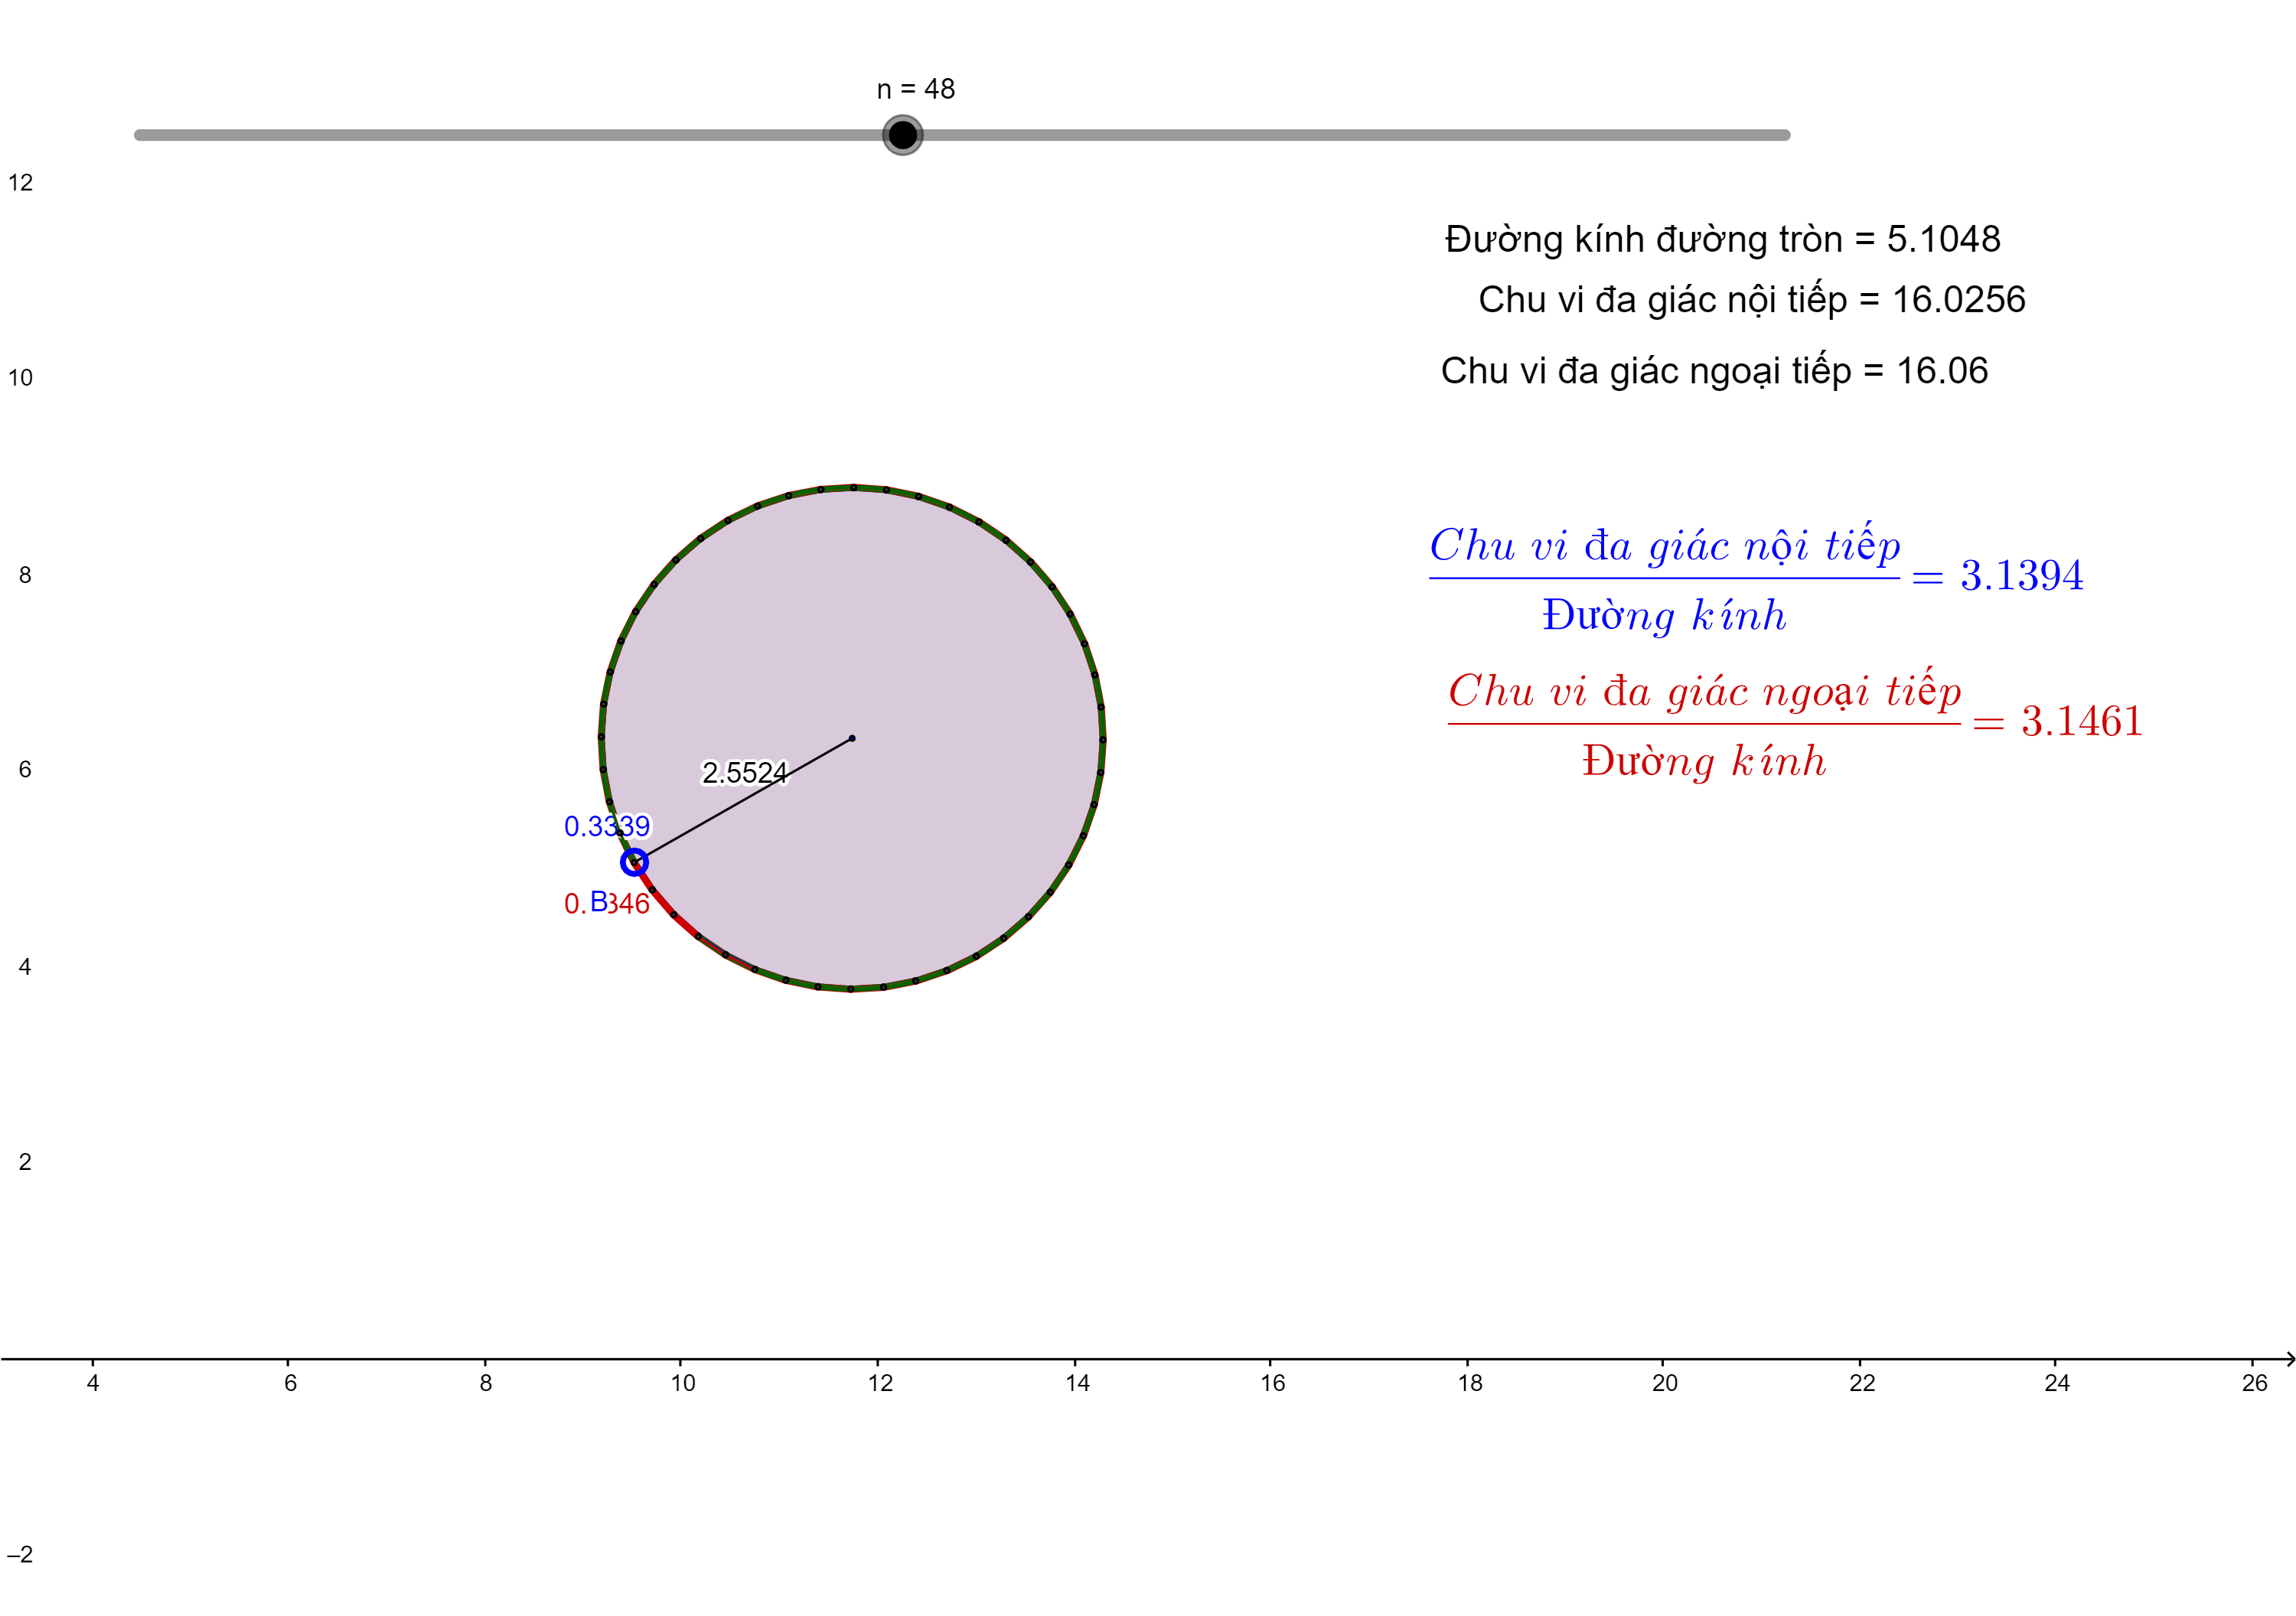
\includegraphics[width= 1\linewidth]{15}
%		\caption{\small\textit{\color{lichsutoanhoc}$n = 48$.}}
%		\vspace*{-10pt}
%	\end{figure}
	\begin{figure}[H]
		\vspace*{-5pt}
		\centering
		\captionsetup{labelformat= empty, justification=centering}
		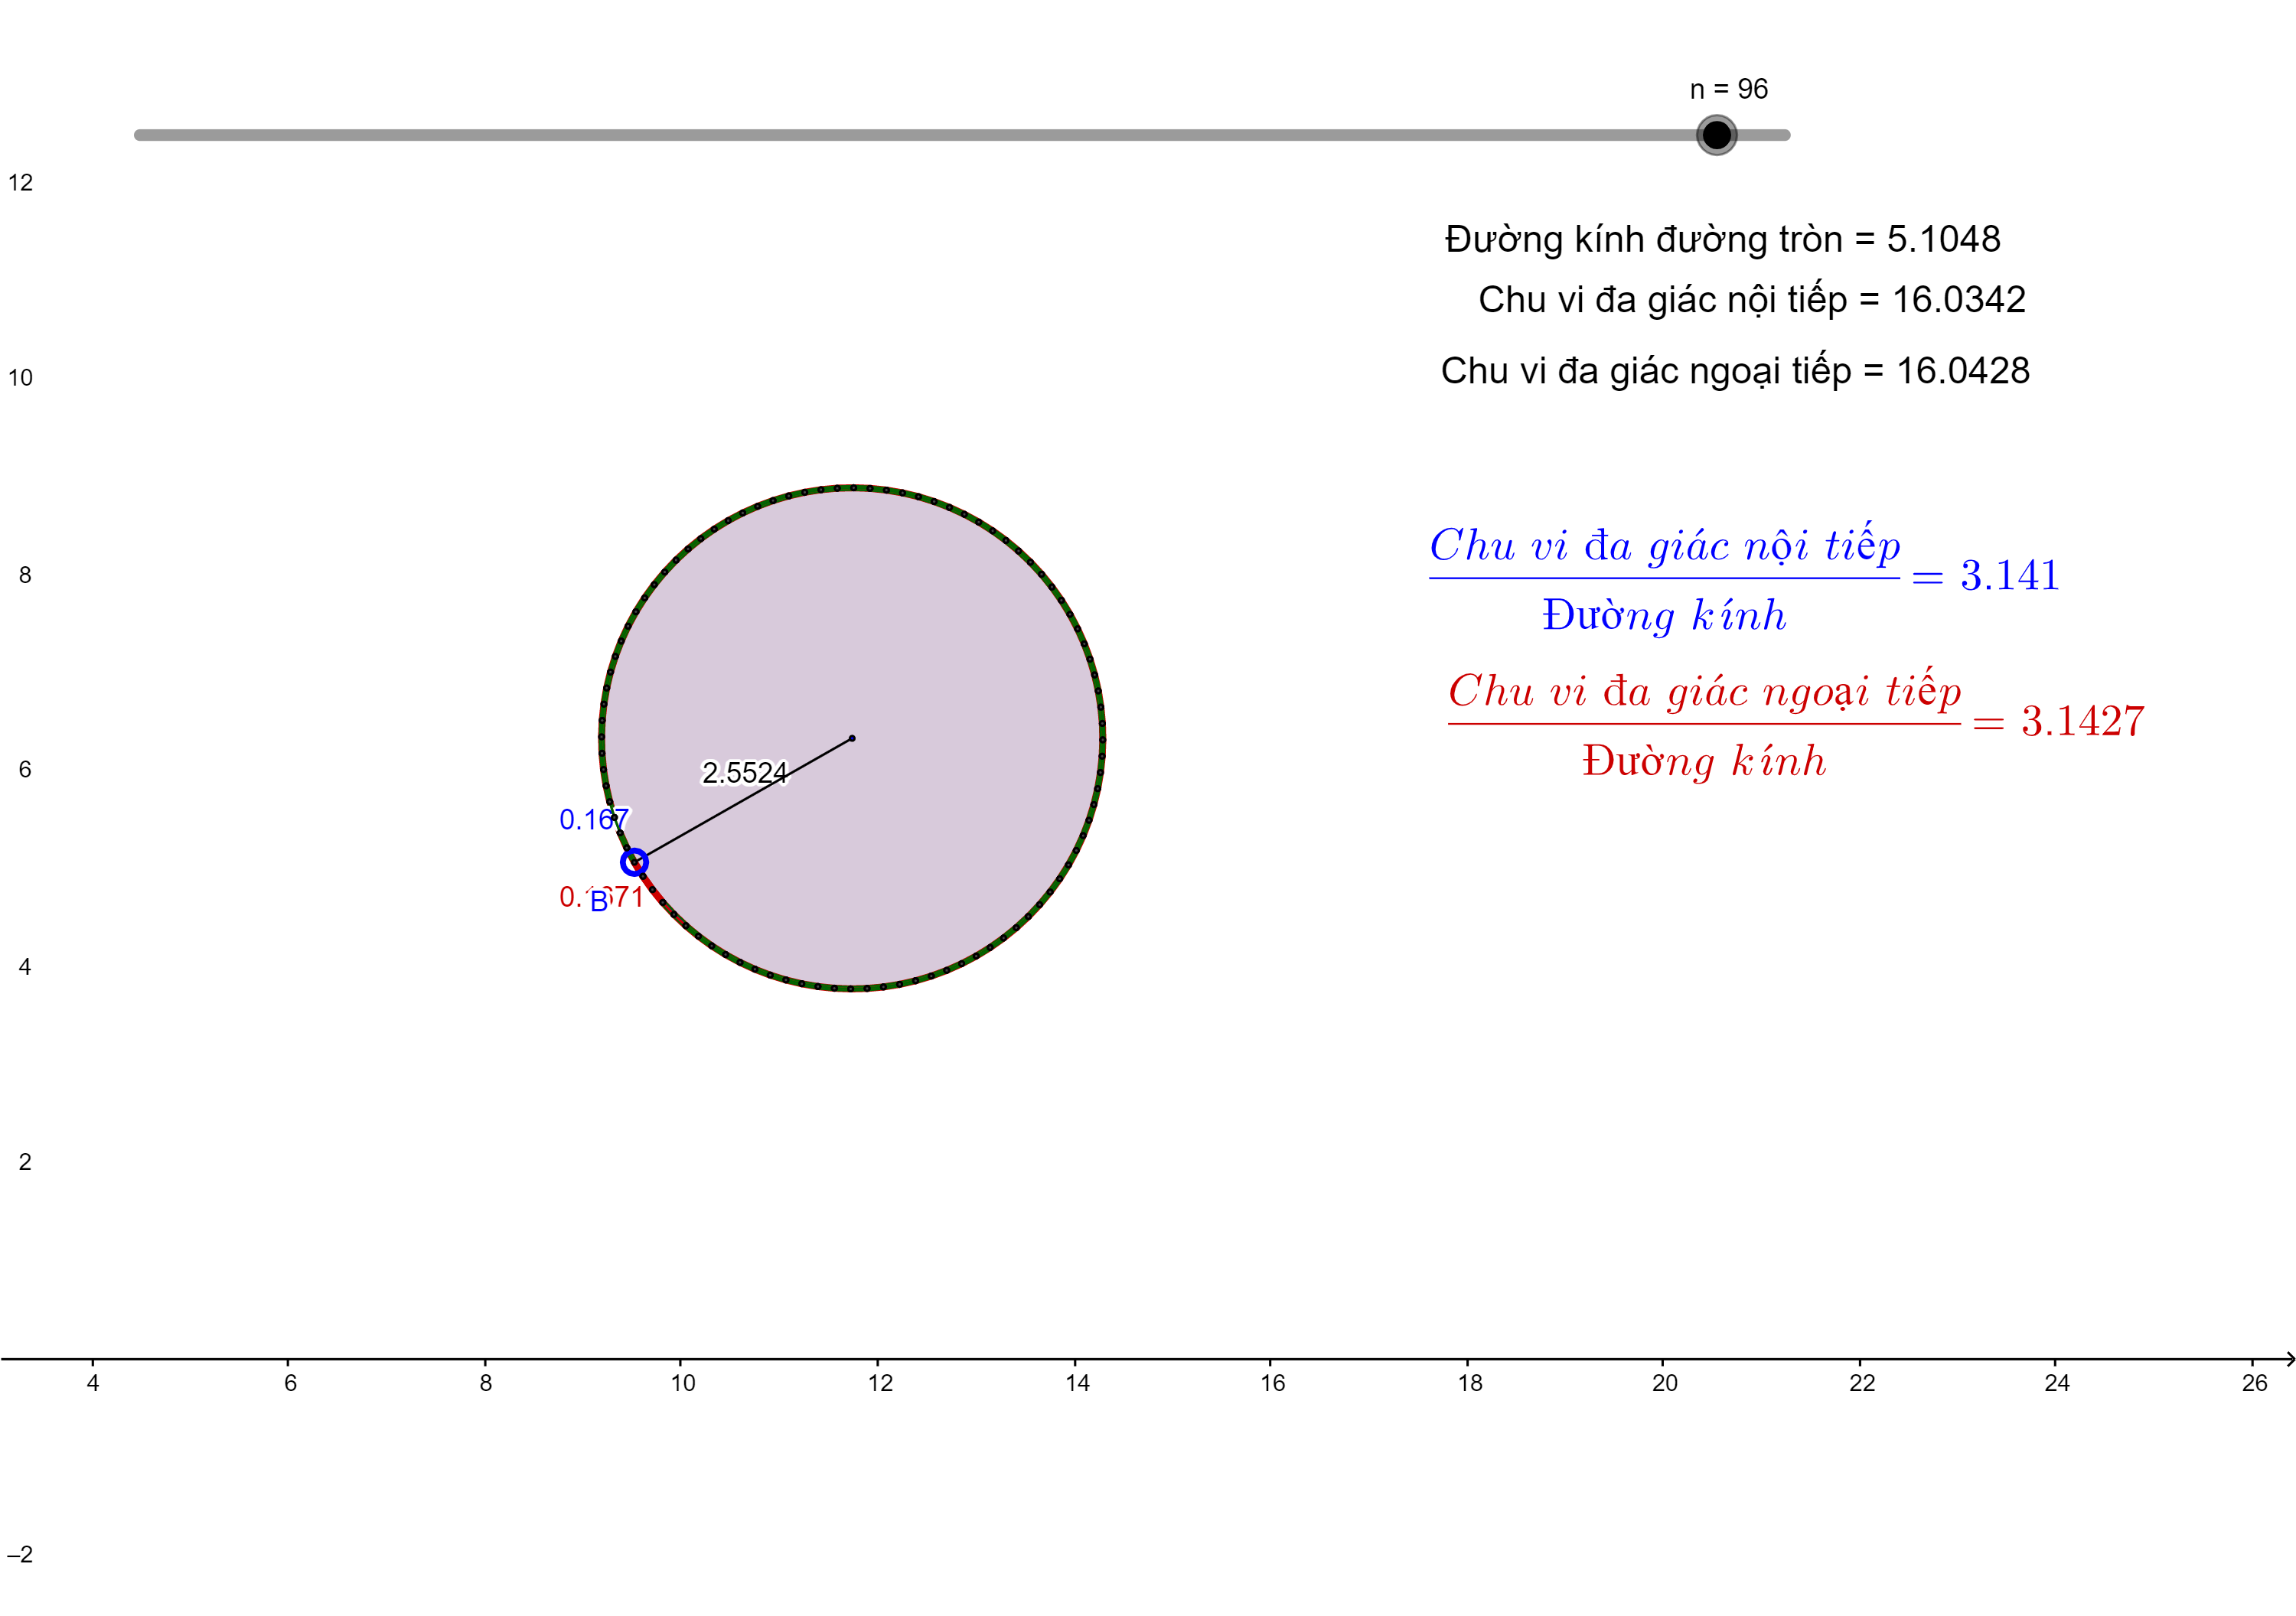
\includegraphics[width= 1\linewidth]{16}
		\caption{\small\textit{\color{lichsutoanhoc}$n = 96$.}}
		\vspace*{-10pt}
	\end{figure}	
	\textit{GeoGebra} đã cài đặt số Pi gần đúng đến $13$ chữ số $3{,}141592653589$.
	\vskip 0.1cm  
	Máy tính điện tử khoa học (Casio fx--$580$) đã cài đặt số Pi gần đúng đến $10$ chữ số
	\begin{align*}
		\pi \approx 3{,}141592653
	\end{align*}
	\textbf{\color{lichsutoanhoc}Thay lời kết}
	\vskip 0.1cm
	Xung quanh số $\pi$  còn khá nhiều điều đáng được quan tâm. Thí dụ:
	\vskip 0.1cm
	$1)$ Tính chất vô tỷ và siêu việt (không là nghiệm của phương trình đa thức) của số $\pi$.
	\vskip 0.1cm  
	$2)$ Biểu diễn số  $\pi$ qua phân số liên tục.
	\vskip 0.1cm
	$3)$ Các công thức mới, lập trình và tính gần đúng số $\pi$  trên các máy tính hiện đại. 
	\vskip 0.1cm
	$4)$ Phương pháp Monte--Carlo tính gần đúng $\pi$.
	\vskip 0.1cm   
	$5)$ Số $\pi$ và những vấn đề toán học liên quan (Công thức Euler, Hàm zeta, Fractal, \ldots).
	\vskip 0.1cm
	$6)$ Số $\pi$ trong cuộc sống, \ldots 
	\vskip 0.1cm
	Bạn đọc có thể tham khảo thêm trong các tài liệu [$2$], [$3$]  và trên Internet. 
	\vskip 0.1cm
	\textbf{\color{lichsutoanhoc}Tài liệu tham khảo}
	\vskip 0.1cm
	[$1$] Tạ Duy Phượng, Đoàn Thị Lệ, Cung Thị Kim Thành, Mai Văn Thu, Nguyễn Hoàng Vũ, Tính số Pi: Xưa và Nay, Phần $1$: Tính số Pi: Xưa, Tạp chí Pi, Tập $7$, số $3$, $2023$.
	\vskip 0.1cm
	[$2$] Petr Beckmann, \textit{A History of} $\pi$ (Pi), St. Martin's Press, New York, in lần thứ ba, $1974$.
	\vskip 0.1cm 
	[$3$] Lennart Berggren, Jonathan Borwein, Peter Borwein, Pi: \textit{A Source Book} (Second Edition), Springer, $2000$.
	\vskip 0.1cm 
	[$4$] Một số tư liệu trên Internet.
\end{multicols}